% Options for packages loaded elsewhere
\PassOptionsToPackage{unicode}{hyperref}
\PassOptionsToPackage{hyphens}{url}
\PassOptionsToPackage{dvipsnames,svgnames,x11names}{xcolor}
%
\documentclass[
  letterpaper,
  DIV=11,
  numbers=noendperiod]{scrartcl}

\usepackage{amsmath,amssymb}
\usepackage{iftex}
\ifPDFTeX
  \usepackage[T1]{fontenc}
  \usepackage[utf8]{inputenc}
  \usepackage{textcomp} % provide euro and other symbols
\else % if luatex or xetex
  \usepackage{unicode-math}
  \defaultfontfeatures{Scale=MatchLowercase}
  \defaultfontfeatures[\rmfamily]{Ligatures=TeX,Scale=1}
\fi
\usepackage{lmodern}
\ifPDFTeX\else  
    % xetex/luatex font selection
\fi
% Use upquote if available, for straight quotes in verbatim environments
\IfFileExists{upquote.sty}{\usepackage{upquote}}{}
\IfFileExists{microtype.sty}{% use microtype if available
  \usepackage[]{microtype}
  \UseMicrotypeSet[protrusion]{basicmath} % disable protrusion for tt fonts
}{}
\makeatletter
\@ifundefined{KOMAClassName}{% if non-KOMA class
  \IfFileExists{parskip.sty}{%
    \usepackage{parskip}
  }{% else
    \setlength{\parindent}{0pt}
    \setlength{\parskip}{6pt plus 2pt minus 1pt}}
}{% if KOMA class
  \KOMAoptions{parskip=half}}
\makeatother
\usepackage{xcolor}
\setlength{\emergencystretch}{3em} % prevent overfull lines
\setcounter{secnumdepth}{5}
% Make \paragraph and \subparagraph free-standing
\ifx\paragraph\undefined\else
  \let\oldparagraph\paragraph
  \renewcommand{\paragraph}[1]{\oldparagraph{#1}\mbox{}}
\fi
\ifx\subparagraph\undefined\else
  \let\oldsubparagraph\subparagraph
  \renewcommand{\subparagraph}[1]{\oldsubparagraph{#1}\mbox{}}
\fi


\providecommand{\tightlist}{%
  \setlength{\itemsep}{0pt}\setlength{\parskip}{0pt}}\usepackage{longtable,booktabs,array}
\usepackage{calc} % for calculating minipage widths
% Correct order of tables after \paragraph or \subparagraph
\usepackage{etoolbox}
\makeatletter
\patchcmd\longtable{\par}{\if@noskipsec\mbox{}\fi\par}{}{}
\makeatother
% Allow footnotes in longtable head/foot
\IfFileExists{footnotehyper.sty}{\usepackage{footnotehyper}}{\usepackage{footnote}}
\makesavenoteenv{longtable}
\usepackage{graphicx}
\makeatletter
\def\maxwidth{\ifdim\Gin@nat@width>\linewidth\linewidth\else\Gin@nat@width\fi}
\def\maxheight{\ifdim\Gin@nat@height>\textheight\textheight\else\Gin@nat@height\fi}
\makeatother
% Scale images if necessary, so that they will not overflow the page
% margins by default, and it is still possible to overwrite the defaults
% using explicit options in \includegraphics[width, height, ...]{}
\setkeys{Gin}{width=\maxwidth,height=\maxheight,keepaspectratio}
% Set default figure placement to htbp
\makeatletter
\def\fps@figure{htbp}
\makeatother

\usepackage{booktabs}
\usepackage{caption}
\usepackage{longtable}
\usepackage{colortbl}
\usepackage{array}
\usepackage{anyfontsize}
\usepackage{multirow}
\KOMAoption{captions}{tableheading}
\makeatletter
\@ifpackageloaded{caption}{}{\usepackage{caption}}
\AtBeginDocument{%
\ifdefined\contentsname
  \renewcommand*\contentsname{Table of contents}
\else
  \newcommand\contentsname{Table of contents}
\fi
\ifdefined\listfigurename
  \renewcommand*\listfigurename{List of Figures}
\else
  \newcommand\listfigurename{List of Figures}
\fi
\ifdefined\listtablename
  \renewcommand*\listtablename{List of Tables}
\else
  \newcommand\listtablename{List of Tables}
\fi
\ifdefined\figurename
  \renewcommand*\figurename{Figure}
\else
  \newcommand\figurename{Figure}
\fi
\ifdefined\tablename
  \renewcommand*\tablename{Table}
\else
  \newcommand\tablename{Table}
\fi
}
\@ifpackageloaded{float}{}{\usepackage{float}}
\floatstyle{ruled}
\@ifundefined{c@chapter}{\newfloat{codelisting}{h}{lop}}{\newfloat{codelisting}{h}{lop}[chapter]}
\floatname{codelisting}{Listing}
\newcommand*\listoflistings{\listof{codelisting}{List of Listings}}
\makeatother
\makeatletter
\makeatother
\makeatletter
\@ifpackageloaded{caption}{}{\usepackage{caption}}
\@ifpackageloaded{subcaption}{}{\usepackage{subcaption}}
\makeatother
\ifLuaTeX
  \usepackage{selnolig}  % disable illegal ligatures
\fi
\usepackage{bookmark}

\IfFileExists{xurl.sty}{\usepackage{xurl}}{} % add URL line breaks if available
\urlstyle{same} % disable monospaced font for URLs
\hypersetup{
  pdftitle={U.S. EPA National Sewershed Dataset \& Model Documentation},
  colorlinks=true,
  linkcolor={blue},
  filecolor={Maroon},
  citecolor={Blue},
  urlcolor={Blue},
  pdfcreator={LaTeX via pandoc}}

\title{U.S. EPA National Sewershed Dataset \& Model Documentation}
\author{}
\date{}

\begin{document}
\maketitle

\renewcommand*\contentsname{Table of contents}
{
\hypersetup{linkcolor=}
\setcounter{tocdepth}{3}
\tableofcontents
}
This document serves as background material for the EPA National
Sewershed Dataset. The dataset can be accessed via the
\href{https://epa.maps.arcgis.com/apps/instant/atlas/index.html?appid=5b098638234349dd8dca7f764e7aa4e3}{EPA
internal web application}

\subsection{Executive Summary}\label{executive-summary}

\begin{quote}
``The
\href{https://www.epa.gov/cwns/clean-watersheds-needs-survey-cwns-2022-report-and-data}{Clean
Watershed Needs Survey(CWNS)}provides an assessment of the capital
investments necessary for states, the District of Columbia, and U.S.
Territories to meet the Clean Water Act's (CWA) water quality goals over
the subsequent 20 years. These needs include projects and related
infrastructure costs for wastewater publicly owned treatment works,
stormwater treatment, nonpoint source control, and decentralized
wastewater treatment. The U.S. Environmental Protection Agency (EPA) has
prepared the 2022 CWNS Report to Congress in compliance with CWA section
516(b)(1)(B) (33 U.S Code §1375) as well as CWA section 609, which was
added by the Infrastructure Investment and Jobs Act (IIJA), P.L. 117-58,
November 15, 2021. This Report summarizes the results of EPA's 17th
survey since the CWA was enacted in 1972.''
\end{quote}

As part of this survey, utilities submit information related to their
treatment plants. Some treatment plants may discharge a portion of their
wastewater downstream to other treatment plants. When a treatment plant
discharges less than 50\% of its wastewater to another facility, we
refer to it as an `endpoint', meaning that it is considered the final
destination for wastewater prior to treatment and then discharge back
into the environment, most frequently via direct discharge into a water
body such as a river or ocean. The entire sewered area that contributes
wastewater to a specific endpoint is referred to as a `sewershed'. A
sewershed may therfore refer to a system that is smaller than a single
utility or conversely be made up of multiple utilities. The relationship
between utilities and endpoints can be derived from CWNS reporting by
accounting for reported discharge of wastewater between facilities.

Sewershed extents are not a part of reporting within the CWNS and are
otherwise not statutorily required under the CWA. Understanding the
sewered area related to an endpoint however, is critical to support the
CWA, as well as multiple other agency and administration priorities.
Sewershed boundaries can, for example, facilitate wastewater
surveillance efforts and link disease tracking to affected populations.
The ability to map sewer systems can also be critical to infrastructure
and urban planning, providing information on areas that can be developed
or could benefit from resources to aid in economic development.

EPA previously developed geospatial data for community water system
service areas for the United States. The development of sewershed
boundaries was built off of this experience, using machine learning
models which are trained on existing sewershed data and utilizing
advanced geospatial techniques to account for the complexities of
determining what areas of the United States are sewered and which
treatment plants they are served by. The output of this dataset is a
spatial dataset of polygons that are constructed from hexagons with a
resolution of \textasciitilde0.11 km\textsuperscript{2}

\subsection{Introduction}\label{introduction}

Prior modeling similar to sewershed was conducted by EPA in 2024 for the
service areas of community water systems. While there are many
similarities between public water and wastewater infrastructure, there
are several key differences. For example, there are more than twice as
many community water systems in the United States as there are publicly
owned treatment works (POTWs). In general, sewer systems represent a
larger investment in infrastructure than public water service. Water,
for example, is pressurized throughout the system and can more easily
overcome changes in topography, whereas sewer largely relies on gravity
for wastewater flow. Where gravity must be overcome within wastewater
systems, pumping or elevator stations must be installed. Sewer lines are
also larger than water supply lines and come with increased construction
costs. It is not uncommon for a suburban or rural home to have a public
water connection for supply and a septic system for discharge of
wastewater. However, having access to a sewer and no access to public
water occurs far more infrequently. This suggests that sewer systems are
more frequently located in more urbanized areas.

The previous model for community water systems utilized census blocks,
supplemented with land parcels as the basic building block for service
areas. We have changed the spatial unit for this model to
\href{https://h3geo.org/}{H3 hexagons}. H3 hexagons are a global grid
system that have several key advantages over census boundaries. For
example, because hexagons are roughly the same size anywhere on the
planet, many statistical computations related to area and distance can
be streamlined, which allows for the development of predictor variables
that can incorporate more complexity into machine learning models. The
level of resolution we chose for the sewershed model was level 9, which
is roughly 0.11 km\textsuperscript{2}. Incoporating additional
complexity into our predictive data, we also advanced the model from a
random forest (used for community water systems) to a boosted tree
method, which allows for more confidence in the model predictions and
the ability to better determine relationships among predictor data that
may have otherwise been obscured.

This document provides detail on how public data was collected, how the
model was developed and discusses the resulting national dataset of
sewersheds and how it can be used to support EPA's mission.

\subsection{Definitions}\label{definitions}

\begin{longtable}[]{@{}
  >{\raggedright\arraybackslash}p{(\columnwidth - 2\tabcolsep) * \real{0.3333}}
  >{\raggedright\arraybackslash}p{(\columnwidth - 2\tabcolsep) * \real{0.6667}}@{}}
\toprule\noalign{}
\begin{minipage}[b]{\linewidth}\raggedright
Term
\end{minipage} & \begin{minipage}[b]{\linewidth}\raggedright
Definition
\end{minipage} \\
\midrule\noalign{}
\endhead
\bottomrule\noalign{}
\endlastfoot
CWNS & Clean Watershed Needs Survey \\
Endpoint & The point of convergence for all wastewater collected within
a `sewershed' \\
Sewershed & The area that contributes wastewater to a specific
endpoint \\
Utility & A public or private entity that provides wastewater treatment
services \\
POTW & Publicly Owned Treatment Works \\
\end{longtable}

\subsection{Existing Sewershed Data}\label{existing-sewershed-data}

The goal of this project was to publish a comprehensive dataset of
sewershed boundaries in the United States that can be linked to the
CWNS. To that end, we sought to include as many publicly available
sewershed areas as possible. Ideally, every boundary would be sourced
from the utility level to represent the most accurate representation of
sewersheds possible. However, this data does not always exist, which
necessitates the creation of modeling approaches to fill in the gaps.

EPA conducted a rigorous search for publicly available sewershed data
through online searches and engagement with stakeholders including
federal and state agencies, regional partners, NGOs and academics
working in the wastewater field. In total, we obtained 3,280 sewersheds
from public sources which could be linked to the CWNS
(Table~\ref{tbl-stateSwr}).

\begin{table}

\caption{\label{tbl-stateSwr}The total number of publicly available
sewershed areas obtained by EPA for inclusion in the final dataset and
for consideration in model training and testing.}

\centering{

\fontsize{12.0pt}{14.4pt}\selectfont
\begin{tabular*}{\linewidth}{@{\extracolsep{\fill}}>{\raggedright\arraybackslash}p{\dimexpr 75.00pt -2\tabcolsep-1.5\arrayrulewidth}>{\centering\arraybackslash}p{\dimexpr 75.00pt -2\tabcolsep-1.5\arrayrulewidth}>{\centering\arraybackslash}p{\dimexpr 75.00pt -2\tabcolsep-1.5\arrayrulewidth}>{\raggedright\arraybackslash}p{\dimexpr 150.00pt -2\tabcolsep-1.5\arrayrulewidth}>{\raggedright\arraybackslash}p{\dimexpr 150.00pt -2\tabcolsep-1.5\arrayrulewidth}}
\toprule
State & Sewered Population of Utility Sourced Sewersheds & Count of Utility Sourced Sewersheds & \% of State Sewersheds & \% of Sewered Population Served by Utility Sourced Sewersheds \\ 
\midrule\addlinespace[2.5pt]
Arizona & 824,116 & 7 & <div style='flex-grow:1;margin-left:8px;background:#e1e1e1;'><div style='background:#4f97d1;width:6%;height:16px;display:flex;align-items:center;justify-content:center;color:#000000;font-weight:bold;font-size:10px;position:relative;'><span style='color:#000000;position:absolute;left:0%;margin-left:6px;font-weight:bold;font-size:10px;'>6%</span></div></div> & <div style='flex-grow:1;margin-left:8px;background:#e1e1e1;'><div style='background:#4f97d1;width:16%;height:16px;display:flex;align-items:center;justify-content:center;color:#000000;font-weight:bold;font-size:10px;position:relative;'><span style='color:#000000;position:absolute;left:0%;margin-left:16px;font-weight:bold;font-size:10px;'>16%</span></div></div> \\ 
Arkansas & 130,389 & 1 & <div style='flex-grow:1;margin-left:8px;background:#e1e1e1;'><div style='background:#4f97d1;width:0%;height:16px;display:flex;align-items:center;justify-content:center;color:#000000;font-weight:bold;font-size:10px;position:relative;'><span style='color:#000000;position:absolute;left:0%;margin-left:0px;font-weight:bold;font-size:10px;'>0%</span></div></div> & <div style='flex-grow:1;margin-left:8px;background:#e1e1e1;'><div style='background:#4f97d1;width:7%;height:16px;display:flex;align-items:center;justify-content:center;color:#000000;font-weight:bold;font-size:10px;position:relative;'><span style='color:#000000;position:absolute;left:0%;margin-left:7px;font-weight:bold;font-size:10px;'>7%</span></div></div> \\ 
California & 1,285,642 & 26 & <div style='flex-grow:1;margin-left:8px;background:#e1e1e1;'><div style='background:#4f97d1;width:5%;height:16px;display:flex;align-items:center;justify-content:center;color:#000000;font-weight:bold;font-size:10px;position:relative;'><span style='color:#000000;position:absolute;left:0%;margin-left:5px;font-weight:bold;font-size:10px;'>5%</span></div></div> & <div style='flex-grow:1;margin-left:8px;background:#e1e1e1;'><div style='background:#4f97d1;width:3%;height:16px;display:flex;align-items:center;justify-content:center;color:#000000;font-weight:bold;font-size:10px;position:relative;'><span style='color:#000000;position:absolute;left:0%;margin-left:3px;font-weight:bold;font-size:10px;'>3%</span></div></div> \\ 
Colorado & 876,568 & 72 & <div style='flex-grow:1;margin-left:8px;background:#e1e1e1;'><div style='background:#4f97d1;width:18%;height:16px;display:flex;align-items:center;justify-content:center;color:#000000;font-weight:bold;font-size:10px;position:relative;'><span style='color:#000000;position:absolute;left:0%;margin-left:18px;font-weight:bold;font-size:10px;'>18%</span></div></div> & <div style='flex-grow:1;margin-left:8px;background:#e1e1e1;'><div style='background:#4f97d1;width:15%;height:16px;display:flex;align-items:center;justify-content:center;color:#000000;font-weight:bold;font-size:10px;position:relative;'><span style='color:#000000;position:absolute;left:0%;margin-left:15px;font-weight:bold;font-size:10px;'>15%</span></div></div> \\ 
Connecticut & 2,803,707 & 80 & <div style='flex-grow:1;margin-left:8px;background:#e1e1e1;'><div style='background:#4f97d1;width:87%;height:16px;display:flex;align-items:center;justify-content:flex-start;position:relative;'><span style='color:#000000;position:absolute;left:0px;margin-left:5px;font-weight:bold;font-size:10px;'>87%</span></div></div> & <div style='flex-grow:1;margin-left:8px;background:#e1e1e1;'><div style='background:#4f97d1;width:92%;height:16px;display:flex;align-items:center;justify-content:flex-start;position:relative;'><span style='color:#000000;position:absolute;left:0px;margin-left:5px;font-weight:bold;font-size:10px;'>92%</span></div></div> \\ 
Delaware & 561,514 & 7 & <div style='flex-grow:1;margin-left:8px;background:#e1e1e1;'><div style='background:#4f97d1;width:41%;height:16px;display:flex;align-items:center;justify-content:flex-start;position:relative;'><span style='color:#000000;position:absolute;left:0px;margin-left:5px;font-weight:bold;font-size:10px;'>41%</span></div></div> & <div style='flex-grow:1;margin-left:8px;background:#e1e1e1;'><div style='background:#4f97d1;width:71%;height:16px;display:flex;align-items:center;justify-content:flex-start;position:relative;'><span style='color:#000000;position:absolute;left:0px;margin-left:5px;font-weight:bold;font-size:10px;'>71%</span></div></div> \\ 
District of Columbia & 2,016,161 & 1 & <div style='flex-grow:1;margin-left:8px;background:#e1e1e1;'><div style='background:#4f97d1;width:100%;height:16px;display:flex;align-items:center;justify-content:flex-start;position:relative;'><span style='color:#000000;position:absolute;left:0px;margin-left:5px;font-weight:bold;font-size:10px;'>100%</span></div></div> & <div style='flex-grow:1;margin-left:8px;background:#e1e1e1;'><div style='background:#4f97d1;width:100%;height:16px;display:flex;align-items:center;justify-content:flex-start;position:relative;'><span style='color:#000000;position:absolute;left:0px;margin-left:5px;font-weight:bold;font-size:10px;'>100%</span></div></div> \\ 
Florida & 8,423,589 & 153 & <div style='flex-grow:1;margin-left:8px;background:#e1e1e1;'><div style='background:#4f97d1;width:41%;height:16px;display:flex;align-items:center;justify-content:flex-start;position:relative;'><span style='color:#000000;position:absolute;left:0px;margin-left:5px;font-weight:bold;font-size:10px;'>41%</span></div></div> & <div style='flex-grow:1;margin-left:8px;background:#e1e1e1;'><div style='background:#4f97d1;width:49%;height:16px;display:flex;align-items:center;justify-content:flex-start;position:relative;'><span style='color:#000000;position:absolute;left:0px;margin-left:5px;font-weight:bold;font-size:10px;'>49%</span></div></div> \\ 
Georgia & 187,539 & 16 & <div style='flex-grow:1;margin-left:8px;background:#e1e1e1;'><div style='background:#4f97d1;width:4%;height:16px;display:flex;align-items:center;justify-content:center;color:#000000;font-weight:bold;font-size:10px;position:relative;'><span style='color:#000000;position:absolute;left:0%;margin-left:4px;font-weight:bold;font-size:10px;'>4%</span></div></div> & <div style='flex-grow:1;margin-left:8px;background:#e1e1e1;'><div style='background:#4f97d1;width:3%;height:16px;display:flex;align-items:center;justify-content:center;color:#000000;font-weight:bold;font-size:10px;position:relative;'><span style='color:#000000;position:absolute;left:0%;margin-left:3px;font-weight:bold;font-size:10px;'>3%</span></div></div> \\ 
Hawaii & 82,287 & 5 & <div style='flex-grow:1;margin-left:8px;background:#e1e1e1;'><div style='background:#4f97d1;width:23%;height:16px;display:flex;align-items:center;justify-content:center;color:#000000;font-weight:bold;font-size:10px;position:relative;'><span style='color:#000000;position:absolute;left:0%;margin-left:23px;font-weight:bold;font-size:10px;'>23%</span></div></div> & <div style='flex-grow:1;margin-left:8px;background:#e1e1e1;'><div style='background:#4f97d1;width:8%;height:16px;display:flex;align-items:center;justify-content:center;color:#000000;font-weight:bold;font-size:10px;position:relative;'><span style='color:#000000;position:absolute;left:0%;margin-left:8px;font-weight:bold;font-size:10px;'>8%</span></div></div> \\ 
Illinois & 1,807,064 & 37 & <div style='flex-grow:1;margin-left:8px;background:#e1e1e1;'><div style='background:#4f97d1;width:5%;height:16px;display:flex;align-items:center;justify-content:center;color:#000000;font-weight:bold;font-size:10px;position:relative;'><span style='color:#000000;position:absolute;left:0%;margin-left:5px;font-weight:bold;font-size:10px;'>5%</span></div></div> & <div style='flex-grow:1;margin-left:8px;background:#e1e1e1;'><div style='background:#4f97d1;width:16%;height:16px;display:flex;align-items:center;justify-content:center;color:#000000;font-weight:bold;font-size:10px;position:relative;'><span style='color:#000000;position:absolute;left:0%;margin-left:16px;font-weight:bold;font-size:10px;'>16%</span></div></div> \\ 
Iowa & 749,994 & 2 & <div style='flex-grow:1;margin-left:8px;background:#e1e1e1;'><div style='background:#4f97d1;width:0%;height:16px;display:flex;align-items:center;justify-content:center;color:#000000;font-weight:bold;font-size:10px;position:relative;'><span style='color:#000000;position:absolute;left:0%;margin-left:0px;font-weight:bold;font-size:10px;'>0%</span></div></div> & <div style='flex-grow:1;margin-left:8px;background:#e1e1e1;'><div style='background:#4f97d1;width:28%;height:16px;display:flex;align-items:center;justify-content:center;color:#000000;font-weight:bold;font-size:10px;position:relative;'><span style='color:#000000;position:absolute;left:0%;margin-left:28px;font-weight:bold;font-size:10px;'>28%</span></div></div> \\ 
Kansas & 227,797 & 8 & <div style='flex-grow:1;margin-left:8px;background:#e1e1e1;'><div style='background:#4f97d1;width:1%;height:16px;display:flex;align-items:center;justify-content:center;color:#000000;font-weight:bold;font-size:10px;position:relative;'><span style='color:#000000;position:absolute;left:0%;margin-left:1px;font-weight:bold;font-size:10px;'>1%</span></div></div> & <div style='flex-grow:1;margin-left:8px;background:#e1e1e1;'><div style='background:#4f97d1;width:10%;height:16px;display:flex;align-items:center;justify-content:center;color:#000000;font-weight:bold;font-size:10px;position:relative;'><span style='color:#000000;position:absolute;left:0%;margin-left:10px;font-weight:bold;font-size:10px;'>10%</span></div></div> \\ 
Kentucky & 2,042,314 & 228 & <div style='flex-grow:1;margin-left:8px;background:#e1e1e1;'><div style='background:#4f97d1;width:87%;height:16px;display:flex;align-items:center;justify-content:flex-start;position:relative;'><span style='color:#000000;position:absolute;left:0px;margin-left:5px;font-weight:bold;font-size:10px;'>87%</span></div></div> & <div style='flex-grow:1;margin-left:8px;background:#e1e1e1;'><div style='background:#4f97d1;width:70%;height:16px;display:flex;align-items:center;justify-content:flex-start;position:relative;'><span style='color:#000000;position:absolute;left:0px;margin-left:5px;font-weight:bold;font-size:10px;'>70%</span></div></div> \\ 
Maryland & 4,098,834 & 148 & <div style='flex-grow:1;margin-left:8px;background:#e1e1e1;'><div style='background:#4f97d1;width:90%;height:16px;display:flex;align-items:center;justify-content:flex-start;position:relative;'><span style='color:#000000;position:absolute;left:0px;margin-left:5px;font-weight:bold;font-size:10px;'>90%</span></div></div> & <div style='flex-grow:1;margin-left:8px;background:#e1e1e1;'><div style='background:#4f97d1;width:99%;height:16px;display:flex;align-items:center;justify-content:flex-start;position:relative;'><span style='color:#000000;position:absolute;left:0px;margin-left:5px;font-weight:bold;font-size:10px;'>99%</span></div></div> \\ 
Massachusetts & 5,596,970 & 123 & <div style='flex-grow:1;margin-left:8px;background:#e1e1e1;'><div style='background:#4f97d1;width:97%;height:16px;display:flex;align-items:center;justify-content:flex-start;position:relative;'><span style='color:#000000;position:absolute;left:0px;margin-left:5px;font-weight:bold;font-size:10px;'>97%</span></div></div> & <div style='flex-grow:1;margin-left:8px;background:#e1e1e1;'><div style='background:#4f97d1;width:100%;height:16px;display:flex;align-items:center;justify-content:flex-start;position:relative;'><span style='color:#000000;position:absolute;left:0px;margin-left:5px;font-weight:bold;font-size:10px;'>100%</span></div></div> \\ 
Michigan & 2,844,020 & 1 & <div style='flex-grow:1;margin-left:8px;background:#e1e1e1;'><div style='background:#4f97d1;width:0%;height:16px;display:flex;align-items:center;justify-content:center;color:#000000;font-weight:bold;font-size:10px;position:relative;'><span style='color:#000000;position:absolute;left:0%;margin-left:0px;font-weight:bold;font-size:10px;'>0%</span></div></div> & <div style='flex-grow:1;margin-left:8px;background:#e1e1e1;'><div style='background:#4f97d1;width:39%;height:16px;display:flex;align-items:center;justify-content:center;color:#000000;font-weight:bold;font-size:10px;position:relative;'><span style='color:#000000;position:absolute;left:0%;margin-left:39px;font-weight:bold;font-size:10px;'>39%</span></div></div> \\ 
Minnesota & 3,020,783 & 9 & <div style='flex-grow:1;margin-left:8px;background:#e1e1e1;'><div style='background:#4f97d1;width:2%;height:16px;display:flex;align-items:center;justify-content:center;color:#000000;font-weight:bold;font-size:10px;position:relative;'><span style='color:#000000;position:absolute;left:0%;margin-left:2px;font-weight:bold;font-size:10px;'>2%</span></div></div> & <div style='flex-grow:1;margin-left:8px;background:#e1e1e1;'><div style='background:#4f97d1;width:64%;height:16px;display:flex;align-items:center;justify-content:flex-start;position:relative;'><span style='color:#000000;position:absolute;left:0px;margin-left:5px;font-weight:bold;font-size:10px;'>64%</span></div></div> \\ 
Mississippi & 71,368 & 13 & <div style='flex-grow:1;margin-left:8px;background:#e1e1e1;'><div style='background:#4f97d1;width:5%;height:16px;display:flex;align-items:center;justify-content:center;color:#000000;font-weight:bold;font-size:10px;position:relative;'><span style='color:#000000;position:absolute;left:0%;margin-left:5px;font-weight:bold;font-size:10px;'>5%</span></div></div> & <div style='flex-grow:1;margin-left:8px;background:#e1e1e1;'><div style='background:#4f97d1;width:5%;height:16px;display:flex;align-items:center;justify-content:center;color:#000000;font-weight:bold;font-size:10px;position:relative;'><span style='color:#000000;position:absolute;left:0%;margin-left:5px;font-weight:bold;font-size:10px;'>5%</span></div></div> \\ 
Missouri & 5,490,252 & 100 & <div style='flex-grow:1;margin-left:8px;background:#e1e1e1;'><div style='background:#4f97d1;width:12%;height:16px;display:flex;align-items:center;justify-content:center;color:#000000;font-weight:bold;font-size:10px;position:relative;'><span style='color:#000000;position:absolute;left:0%;margin-left:12px;font-weight:bold;font-size:10px;'>12%</span></div></div> & <div style='flex-grow:1;margin-left:8px;background:#e1e1e1;'><div style='background:#4f97d1;width:78%;height:16px;display:flex;align-items:center;justify-content:flex-start;position:relative;'><span style='color:#000000;position:absolute;left:0px;margin-left:5px;font-weight:bold;font-size:10px;'>78%</span></div></div> \\ 
Montana & 115,130 & 10 & <div style='flex-grow:1;margin-left:8px;background:#e1e1e1;'><div style='background:#4f97d1;width:6%;height:16px;display:flex;align-items:center;justify-content:center;color:#000000;font-weight:bold;font-size:10px;position:relative;'><span style='color:#000000;position:absolute;left:0%;margin-left:6px;font-weight:bold;font-size:10px;'>6%</span></div></div> & <div style='flex-grow:1;margin-left:8px;background:#e1e1e1;'><div style='background:#4f97d1;width:19%;height:16px;display:flex;align-items:center;justify-content:center;color:#000000;font-weight:bold;font-size:10px;position:relative;'><span style='color:#000000;position:absolute;left:0%;margin-left:19px;font-weight:bold;font-size:10px;'>19%</span></div></div> \\ 
Nevada & 50,016 & 3 & <div style='flex-grow:1;margin-left:8px;background:#e1e1e1;'><div style='background:#4f97d1;width:5%;height:16px;display:flex;align-items:center;justify-content:center;color:#000000;font-weight:bold;font-size:10px;position:relative;'><span style='color:#000000;position:absolute;left:0%;margin-left:5px;font-weight:bold;font-size:10px;'>5%</span></div></div> & <div style='flex-grow:1;margin-left:8px;background:#e1e1e1;'><div style='background:#4f97d1;width:2%;height:16px;display:flex;align-items:center;justify-content:center;color:#000000;font-weight:bold;font-size:10px;position:relative;'><span style='color:#000000;position:absolute;left:0%;margin-left:2px;font-weight:bold;font-size:10px;'>2%</span></div></div> \\ 
New Hampshire & 669,415 & 61 & <div style='flex-grow:1;margin-left:8px;background:#e1e1e1;'><div style='background:#4f97d1;width:76%;height:16px;display:flex;align-items:center;justify-content:flex-start;position:relative;'><span style='color:#000000;position:absolute;left:0px;margin-left:5px;font-weight:bold;font-size:10px;'>76%</span></div></div> & <div style='flex-grow:1;margin-left:8px;background:#e1e1e1;'><div style='background:#4f97d1;width:91%;height:16px;display:flex;align-items:center;justify-content:flex-start;position:relative;'><span style='color:#000000;position:absolute;left:0px;margin-left:5px;font-weight:bold;font-size:10px;'>91%</span></div></div> \\ 
New Jersey & 8,395,883 & 150 & <div style='flex-grow:1;margin-left:8px;background:#e1e1e1;'><div style='background:#4f97d1;width:94%;height:16px;display:flex;align-items:center;justify-content:flex-start;position:relative;'><span style='color:#000000;position:absolute;left:0px;margin-left:5px;font-weight:bold;font-size:10px;'>94%</span></div></div> & <div style='flex-grow:1;margin-left:8px;background:#e1e1e1;'><div style='background:#4f97d1;width:99%;height:16px;display:flex;align-items:center;justify-content:flex-start;position:relative;'><span style='color:#000000;position:absolute;left:0px;margin-left:5px;font-weight:bold;font-size:10px;'>99%</span></div></div> \\ 
New Mexico & 143,229 & 2 & <div style='flex-grow:1;margin-left:8px;background:#e1e1e1;'><div style='background:#4f97d1;width:2%;height:16px;display:flex;align-items:center;justify-content:center;color:#000000;font-weight:bold;font-size:10px;position:relative;'><span style='color:#000000;position:absolute;left:0%;margin-left:2px;font-weight:bold;font-size:10px;'>2%</span></div></div> & <div style='flex-grow:1;margin-left:8px;background:#e1e1e1;'><div style='background:#4f97d1;width:10%;height:16px;display:flex;align-items:center;justify-content:center;color:#000000;font-weight:bold;font-size:10px;position:relative;'><span style='color:#000000;position:absolute;left:0%;margin-left:10px;font-weight:bold;font-size:10px;'>10%</span></div></div> \\ 
New York & 16,501,156 & 595 & <div style='flex-grow:1;margin-left:8px;background:#e1e1e1;'><div style='background:#4f97d1;width:96%;height:16px;display:flex;align-items:center;justify-content:flex-start;position:relative;'><span style='color:#000000;position:absolute;left:0px;margin-left:5px;font-weight:bold;font-size:10px;'>96%</span></div></div> & <div style='flex-grow:1;margin-left:8px;background:#e1e1e1;'><div style='background:#4f97d1;width:100%;height:16px;display:flex;align-items:center;justify-content:flex-start;position:relative;'><span style='color:#000000;position:absolute;left:0px;margin-left:5px;font-weight:bold;font-size:10px;'>100%</span></div></div> \\ 
North Carolina & 3,466,906 & 225 & <div style='flex-grow:1;margin-left:8px;background:#e1e1e1;'><div style='background:#4f97d1;width:69%;height:16px;display:flex;align-items:center;justify-content:flex-start;position:relative;'><span style='color:#000000;position:absolute;left:0px;margin-left:5px;font-weight:bold;font-size:10px;'>69%</span></div></div> & <div style='flex-grow:1;margin-left:8px;background:#e1e1e1;'><div style='background:#4f97d1;width:51%;height:16px;display:flex;align-items:center;justify-content:flex-start;position:relative;'><span style='color:#000000;position:absolute;left:0px;margin-left:5px;font-weight:bold;font-size:10px;'>51%</span></div></div> \\ 
North Dakota & 140 & 1 & <div style='flex-grow:1;margin-left:8px;background:#e1e1e1;'><div style='background:#4f97d1;width:0%;height:16px;display:flex;align-items:center;justify-content:center;color:#000000;font-weight:bold;font-size:10px;position:relative;'><span style='color:#000000;position:absolute;left:0%;margin-left:0px;font-weight:bold;font-size:10px;'>0%</span></div></div> & <div style='flex-grow:1;margin-left:8px;background:#e1e1e1;'><div style='background:#4f97d1;width:0%;height:16px;display:flex;align-items:center;justify-content:center;color:#000000;font-weight:bold;font-size:10px;position:relative;'><span style='color:#000000;position:absolute;left:0%;margin-left:0px;font-weight:bold;font-size:10px;'>0%</span></div></div> \\ 
Ohio & 5,173,073 & 50 & <div style='flex-grow:1;margin-left:8px;background:#e1e1e1;'><div style='background:#4f97d1;width:6%;height:16px;display:flex;align-items:center;justify-content:center;color:#000000;font-weight:bold;font-size:10px;position:relative;'><span style='color:#000000;position:absolute;left:0%;margin-left:6px;font-weight:bold;font-size:10px;'>6%</span></div></div> & <div style='flex-grow:1;margin-left:8px;background:#e1e1e1;'><div style='background:#4f97d1;width:56%;height:16px;display:flex;align-items:center;justify-content:flex-start;position:relative;'><span style='color:#000000;position:absolute;left:0px;margin-left:5px;font-weight:bold;font-size:10px;'>56%</span></div></div> \\ 
Oklahoma & 128,026 & 1 & <div style='flex-grow:1;margin-left:8px;background:#e1e1e1;'><div style='background:#4f97d1;width:0%;height:16px;display:flex;align-items:center;justify-content:center;color:#000000;font-weight:bold;font-size:10px;position:relative;'><span style='color:#000000;position:absolute;left:0%;margin-left:0px;font-weight:bold;font-size:10px;'>0%</span></div></div> & <div style='flex-grow:1;margin-left:8px;background:#e1e1e1;'><div style='background:#4f97d1;width:4%;height:16px;display:flex;align-items:center;justify-content:center;color:#000000;font-weight:bold;font-size:10px;position:relative;'><span style='color:#000000;position:absolute;left:0%;margin-left:4px;font-weight:bold;font-size:10px;'>4%</span></div></div> \\ 
Oregon & 818,842 & 5 & <div style='flex-grow:1;margin-left:8px;background:#e1e1e1;'><div style='background:#4f97d1;width:2%;height:16px;display:flex;align-items:center;justify-content:center;color:#000000;font-weight:bold;font-size:10px;position:relative;'><span style='color:#000000;position:absolute;left:0%;margin-left:2px;font-weight:bold;font-size:10px;'>2%</span></div></div> & <div style='flex-grow:1;margin-left:8px;background:#e1e1e1;'><div style='background:#4f97d1;width:21%;height:16px;display:flex;align-items:center;justify-content:center;color:#000000;font-weight:bold;font-size:10px;position:relative;'><span style='color:#000000;position:absolute;left:0%;margin-left:21px;font-weight:bold;font-size:10px;'>21%</span></div></div> \\ 
Pennsylvania & 430,629 & 39 & <div style='flex-grow:1;margin-left:8px;background:#e1e1e1;'><div style='background:#4f97d1;width:5%;height:16px;display:flex;align-items:center;justify-content:center;color:#000000;font-weight:bold;font-size:10px;position:relative;'><span style='color:#000000;position:absolute;left:0%;margin-left:5px;font-weight:bold;font-size:10px;'>5%</span></div></div> & <div style='flex-grow:1;margin-left:8px;background:#e1e1e1;'><div style='background:#4f97d1;width:4%;height:16px;display:flex;align-items:center;justify-content:center;color:#000000;font-weight:bold;font-size:10px;position:relative;'><span style='color:#000000;position:absolute;left:0%;margin-left:4px;font-weight:bold;font-size:10px;'>4%</span></div></div> \\ 
Rhode Island & 732,186 & 16 & <div style='flex-grow:1;margin-left:8px;background:#e1e1e1;'><div style='background:#4f97d1;width:80%;height:16px;display:flex;align-items:center;justify-content:flex-start;position:relative;'><span style='color:#000000;position:absolute;left:0px;margin-left:5px;font-weight:bold;font-size:10px;'>80%</span></div></div> & <div style='flex-grow:1;margin-left:8px;background:#e1e1e1;'><div style='background:#4f97d1;width:94%;height:16px;display:flex;align-items:center;justify-content:flex-start;position:relative;'><span style='color:#000000;position:absolute;left:0px;margin-left:5px;font-weight:bold;font-size:10px;'>94%</span></div></div> \\ 
South Carolina & 1,749,700 & 29 & <div style='flex-grow:1;margin-left:8px;background:#e1e1e1;'><div style='background:#4f97d1;width:18%;height:16px;display:flex;align-items:center;justify-content:center;color:#000000;font-weight:bold;font-size:10px;position:relative;'><span style='color:#000000;position:absolute;left:0%;margin-left:18px;font-weight:bold;font-size:10px;'>18%</span></div></div> & <div style='flex-grow:1;margin-left:8px;background:#e1e1e1;'><div style='background:#4f97d1;width:47%;height:16px;display:flex;align-items:center;justify-content:flex-start;position:relative;'><span style='color:#000000;position:absolute;left:0px;margin-left:5px;font-weight:bold;font-size:10px;'>47%</span></div></div> \\ 
Texas & 5,647,426 & 470 & <div style='flex-grow:1;margin-left:8px;background:#e1e1e1;'><div style='background:#4f97d1;width:33%;height:16px;display:flex;align-items:center;justify-content:center;color:#000000;font-weight:bold;font-size:10px;position:relative;'><span style='color:#000000;position:absolute;left:0%;margin-left:33px;font-weight:bold;font-size:10px;'>33%</span></div></div> & <div style='flex-grow:1;margin-left:8px;background:#e1e1e1;'><div style='background:#4f97d1;width:23%;height:16px;display:flex;align-items:center;justify-content:center;color:#000000;font-weight:bold;font-size:10px;position:relative;'><span style='color:#000000;position:absolute;left:0%;margin-left:23px;font-weight:bold;font-size:10px;'>23%</span></div></div> \\ 
Utah & 3,319,337 & 113 & <div style='flex-grow:1;margin-left:8px;background:#e1e1e1;'><div style='background:#4f97d1;width:100%;height:16px;display:flex;align-items:center;justify-content:flex-start;position:relative;'><span style='color:#000000;position:absolute;left:0px;margin-left:5px;font-weight:bold;font-size:10px;'>100%</span></div></div> & <div style='flex-grow:1;margin-left:8px;background:#e1e1e1;'><div style='background:#4f97d1;width:100%;height:16px;display:flex;align-items:center;justify-content:flex-start;position:relative;'><span style='color:#000000;position:absolute;left:0px;margin-left:5px;font-weight:bold;font-size:10px;'>100%</span></div></div> \\ 
Vermont & 323,458 & 92 & <div style='flex-grow:1;margin-left:8px;background:#e1e1e1;'><div style='background:#4f97d1;width:98%;height:16px;display:flex;align-items:center;justify-content:flex-start;position:relative;'><span style='color:#000000;position:absolute;left:0px;margin-left:5px;font-weight:bold;font-size:10px;'>98%</span></div></div> & <div style='flex-grow:1;margin-left:8px;background:#e1e1e1;'><div style='background:#4f97d1;width:100%;height:16px;display:flex;align-items:center;justify-content:flex-start;position:relative;'><span style='color:#000000;position:absolute;left:0px;margin-left:5px;font-weight:bold;font-size:10px;'>100%</span></div></div> \\ 
Virginia & 1,818,789 & 10 & <div style='flex-grow:1;margin-left:8px;background:#e1e1e1;'><div style='background:#4f97d1;width:4%;height:16px;display:flex;align-items:center;justify-content:center;color:#000000;font-weight:bold;font-size:10px;position:relative;'><span style='color:#000000;position:absolute;left:0%;margin-left:4px;font-weight:bold;font-size:10px;'>4%</span></div></div> & <div style='flex-grow:1;margin-left:8px;background:#e1e1e1;'><div style='background:#4f97d1;width:31%;height:16px;display:flex;align-items:center;justify-content:center;color:#000000;font-weight:bold;font-size:10px;position:relative;'><span style='color:#000000;position:absolute;left:0%;margin-left:31px;font-weight:bold;font-size:10px;'>31%</span></div></div> \\ 
Washington & 4,834,886 & 42 & <div style='flex-grow:1;margin-left:8px;background:#e1e1e1;'><div style='background:#4f97d1;width:16%;height:16px;display:flex;align-items:center;justify-content:center;color:#000000;font-weight:bold;font-size:10px;position:relative;'><span style='color:#000000;position:absolute;left:0%;margin-left:16px;font-weight:bold;font-size:10px;'>16%</span></div></div> & <div style='flex-grow:1;margin-left:8px;background:#e1e1e1;'><div style='background:#4f97d1;width:76%;height:16px;display:flex;align-items:center;justify-content:flex-start;position:relative;'><span style='color:#000000;position:absolute;left:0px;margin-left:5px;font-weight:bold;font-size:10px;'>76%</span></div></div> \\ 
West Virginia & 797,007 & 164 & <div style='flex-grow:1;margin-left:8px;background:#e1e1e1;'><div style='background:#4f97d1;width:55%;height:16px;display:flex;align-items:center;justify-content:flex-start;position:relative;'><span style='color:#000000;position:absolute;left:0px;margin-left:5px;font-weight:bold;font-size:10px;'>55%</span></div></div> & <div style='flex-grow:1;margin-left:8px;background:#e1e1e1;'><div style='background:#4f97d1;width:66%;height:16px;display:flex;align-items:center;justify-content:flex-start;position:relative;'><span style='color:#000000;position:absolute;left:0px;margin-left:5px;font-weight:bold;font-size:10px;'>66%</span></div></div> \\ 
Wisconsin & 2,107,614 & 72 & <div style='flex-grow:1;margin-left:8px;background:#e1e1e1;'><div style='background:#4f97d1;width:12%;height:16px;display:flex;align-items:center;justify-content:center;color:#000000;font-weight:bold;font-size:10px;position:relative;'><span style='color:#000000;position:absolute;left:0%;margin-left:12px;font-weight:bold;font-size:10px;'>12%</span></div></div> & <div style='flex-grow:1;margin-left:8px;background:#e1e1e1;'><div style='background:#4f97d1;width:48%;height:16px;display:flex;align-items:center;justify-content:flex-start;position:relative;'><span style='color:#000000;position:absolute;left:0px;margin-left:5px;font-weight:bold;font-size:10px;'>48%</span></div></div> \\ 
\bottomrule
\end{tabular*}

}

\end{table}%

\subsection{Methods}\label{methods}

Three types of tree-based models were considered for this project: a
decision tree, a random forest and boosted trees. All three have
advantages and disadvantages that must be considered. A single decision
tree is the simplest and most easy to interpret method, but can be
overly simplistic and less accurate than more complex models. A random
forest is a collection of decision trees with randomized input
variables, which can improve accuracy and protect from over-fitting but
is less interpretable and requires more computational power. Boosted
trees are a more advanced method that build decisions trees in
succession. Each new decision tree attempts to solve for error found in
the previous tree. This can lead to even better accuracy, but at the
cost of increased complexity and reduced interpretability. Boosted trees
are especially effective at leveraging variables that may otherwise
reflect lower importance levels in other methods. We found that the
higher accuracy returned by boosted tree models justified its selection
over the other two methods. For brevity, only the boosted tree model is
discussed in detail.

\subsubsection{Defining the Universe of
Sewersheds}\label{defining-the-universe-of-sewersheds}

Not all records within the CWNS represent endpoints for wastewater
collection. The first step in our modeling effort is to establish the
universe of systems. To do this, we use the following criteria to select
endpoints:

\begin{itemize}
\tightlist
\item
  POTWs that treat human waste (as opposed to wet weather facilities)\\
\item
  Total receiving population \textgreater{} 0\\
\item
  facility type contains ``treatment plant''
\item
  Residential population \textgreater{} 0
\item
  Percent of Discharge is \textless{} 50\%
\end{itemize}

The data compiled from the CWNS was reviewed for accuracy by
EPA\footnote{After review, it was determined that it is \textbf{NOT}
  safe to assume all rows in `FACILITIES\_CONFIRMED.txt' are all end
  points. It is safe to assume all rows in
  `POPULATION\_WASTEWATER\_CONFIRMED.txt.' are endpoints. rows
  identified as having `CHANGE\_TYPE' = `New' should be removed.}.

The CWNS data we are working with was received as a Microsoft Access
Database, which is located in `Data/CWNS 2022
Database\_April2024.accdb'. We use 7 tables from this access database.
Note that `POPULATION\_WASTEWATER\_CONFIRMED' was manually updated by
ERG in June, 2024 and does not reflect original data in the access
database. Each table was exported from Access to a comma delimited file.
The seven files used are:

\begin{itemize}
\tightlist
\item
  `Data/FACILITIES.txt'
\item
  `Data/POPULATION\_WASTEWATER.txt'
\item
  `Data/FACILITY\_TYPES.txt'
\item
  `Data/PHYSICAL\_LOCATION.txt'
\item
  `Data/FACILITIES\_CONFIRMED.txt'
\item
  `Data/POPULATION\_WASTEWATER\_CONFIRMED\_updated06242024.csv'
\item
  `Data/DISCHARGES.csv'
\end{itemize}

The following steps describe the process used to query endpoints to be
included in modeling efforts. The code can also be viewed in the
expandable code tab.

We create a flat file where each row represents a facility and perform
the followng steps: - In `POPULATION\_WASTEWATER'', if no value is given
for the column 'END\_FACILITY', we assign it ``N'', meaning it is not
considered an end facility. - `END\_FACILITY' and `FACILITY\_TYPE'
columns for the `FACILITIES\_CONFIRMED' file are set to `Y' and
`Treatment Plant' respectively. - Discharge is calculated using the
`DISCHARGES' file. Because systems can discharge to multiple other
systems, we calculate the sum of discharges to determine the total \%
discharged elsewhere. If discharge is not reported for a system, we
default the value to zero. - Data tables are combined and the filter is
applied:

\begin{itemize}
\tightlist
\item
  \texttt{TOTAL\_RES\_POPULATION\_2022\ \textgreater{}\ 0\ \&\ FACILITY\_TYPE=="Treatment\ Plant"\ \&\ PRESENT\_DISCHARGE\_PERCENTAGE\ \textless{}\ 50}
\end{itemize}

Total receiving population = total number of people the facility is
receiving from, regardless of whether its sent on elsewhere

\subsubsection{Matching Utility Sourced Boundaries to CWNS
Locations}\label{matching-utility-sourced-boundaries-to-cwns-locations}

Utility sourced sewersheds had to be matched with their corresponding
CWNS endpoint locations as there is no common identifier between the two
datasets. Matching was done through a combination of spatial
intersections, distance measurements, text similarity between names and
individual visual inspection.

Boundaries were spatially intersected with endpoints. For each match
between a boundary and an endpoint, the total number of endpoints that
intersect a boundary is divided by 1. For example, if only one endpoint
exists within a boundary, the value would be 1. If 3 endpoints intersect
a boundary, the value for all three matches (which are represented as
three separate rows) would be 0.33. This score is labeled `I\_Score' or
\(S_i\)

For boundaries that do not intersect any endpoints, a buffer is applied
using a distance of 16 kilometers, which was found to be the 95\%
confidence level for maximum distance between an endpoint and a service
area (See
`Analysis/Endpoint\_Sewershed\_Distance/Endpoint\_Sewershed\_Distance.html'
for more detailed information). Only endpoints that have not already
been singularly intersected with boundaries are considered in this step.
The distance of each endpoint from the edge of the boundary is divided
by 16 and then subtracted from 1: \(D_{score}=1-(d/16)\), where `d' is
the distance in kilometers. This yields a score such that the closest
endpoint will have the highest score. This score is labeled `D\_Score'
or \(S_d\).

For each pair of matches (CWNS \textless-\textgreater{} State Boundary),
a fuzzy score was calculated to compare the given names of the treatment
works. A score of zero indicates that the names are completely
dissimilar whereas a score of 1 indicates identical names. This score is
labeled `F\_Score' or \(S_f\). The method we use is the `Jaro-Winkler'
distance:

``The Jaro-Winkler distance (method=jw, 0\textless p\textless=0.25) adds
a correction term to the Jaro-distance. It is defined as d − l · p · d,
where d is the Jaro-distance. Here, l is obtained by counting, from the
start of the input strings, after how many characters the first
character mismatch between the two strings occurs, with a maximum of
four. The factor p is a 'prefix' factor, which in the work of Winkler is
often chosen 0.1.''

The Jaro-Winkler method uses 0 for identical and 1 for completely
dissimilar. Therefore: \(S_f=1-D_{JW}\) where \(D_{jw} =\) Jaro-Winkler
Distance

\begin{itemize}
\tightlist
\item
  Scores are aggregated to yield a match score.

  \begin{itemize}
  \tightlist
  \item
    If `I\_Score' is \textgreater{} 0, then the formula we use is:
    \(S_m=S_i+S_f\)
  \item
    If `I\_Score' = 0, we use the formula: \(S_m=S_d+S_f\)
  \end{itemize}
\end{itemize}

This match score equally prioritizes the proximity of an endpoint with
name matching between datasets. In the event that multiple endpoints
intersect a boundary, greater weight is then given to name matching.

\subsubsection{Spatial Resolution}\label{spatial-resolution}

Hexagons were chosen as the spatial unit for the model for several
reasons. Hexagons are roughly the same size across the United States,
they allow for more consistent statistical calculations related to area
and distance and density values do not need to be calculated. Hexagons
also allow for more complex network calculations at higher computation
rates because distance can be inferred as a constant between each
neighboring pair of hexagons. Finally, hexagons offer an advantage to
census blocks, which are delineated based on physical boundaries such as
roads and rivers, which can include undeveloped areas, especially in
rural settings. Using hexagons allows us to create more detailed
sewersheds while reducing overall computation requirements. For this
modeling effort, level 9 hexagons were used, which are
\textasciitilde0.11 km\^{}2 in area.

\begin{figure}

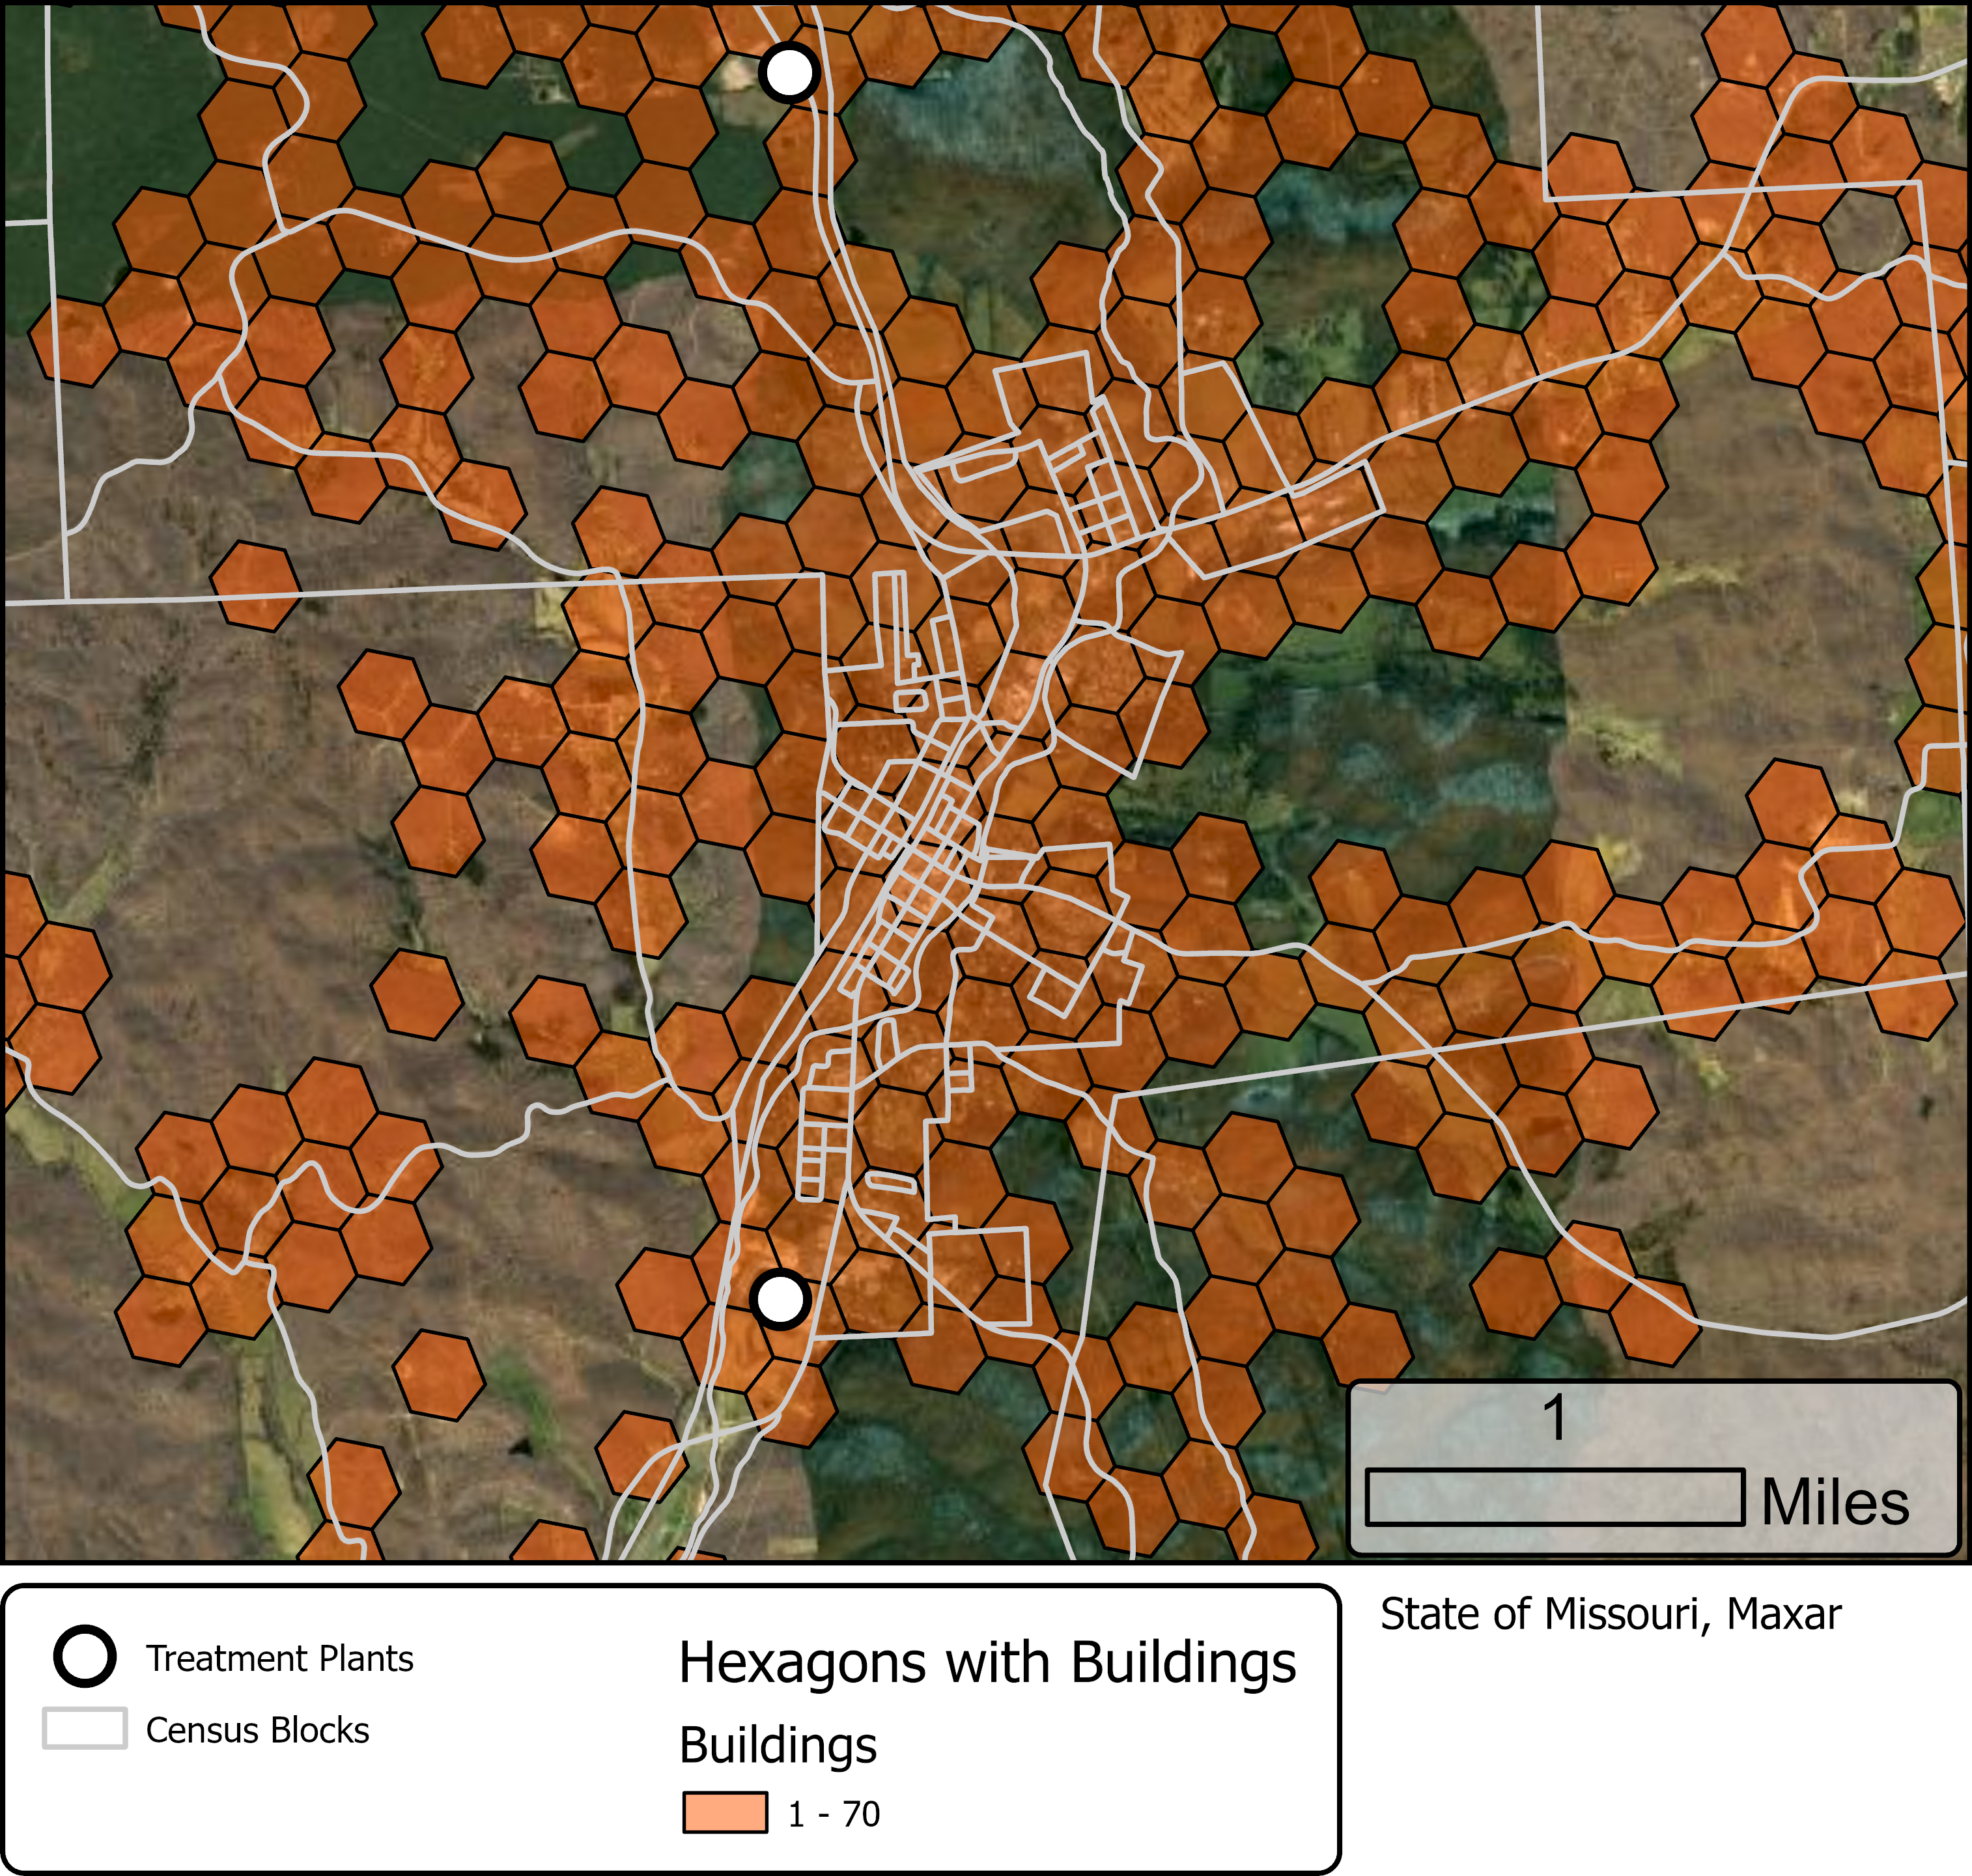
\includegraphics[width=0.5\textwidth,height=\textheight]{img/Hex_Example.png}

\caption{\label{fig-hex}A satelite image of Piedmont, MO illustrating
hexagons with buildings, overlaid by census block boundaries.}

\end{figure}%

\subsubsection{Model Development}\label{model-development}

The goal of the model is to predict whether a hexagon is sewered by a
specific endpoint. Essentially the model is answering two questions.
\textbf{1.} Is the hexagon connected to sewer? and \textbf{2.} If so,
which endpoint is the most likely to serve that hexagon? The model is
therefore a binary classification model, which returns a probability
that a hexagon is part of the sewershed for a given endpoint location.
The model considers each row of a table as a unique pairing between a
specific hexagon and a specific endpoint. Additional data within each
row are the `features' which are predictor variables relating to
physical, environmental and demographic variables unique to that
pairing.

\paragraph{Defining Area of
Consideration}\label{defining-area-of-consideration}

To minimize computation time and increase efficiency, utility sourced
sewersheds were used to test the maximum distance between an endpoint
and the furthest possible hexagon that is served by that endpoint.

\paragraph{Feature Engineering}\label{feature-engineering}

In machine learning, `features' refer to the input data that will act as
predictors for the model. `Feature engineering' therefore refers to the
methods we use to prepare the data so that it contributes to a
successful model. The primary source for the sewershed model is the
CWNS, which includes the locations of treatment plants that are
considered `endpoints', meaning that it is the final stop for wastewater
before being discharged back into the environment. The sewershed is
therefore the entire contributing area that discharges wastewater to
each endpoint.

Sewered areas are typically developed, have relatively dense populations
and are close to a treatment plant. Information fed into the model must
provide relevant tools for relationships to be determined. For example,
sewer systems, unlike public water systems, are generally not
pressurized, meaning that elevation may be a factor. The distance
between a hexagon and a treatment plant may vary depending on how many
people the treatment plant serves. A hexagon with no population, but
with several large buildings and very little green space may indicate an
industrial zone.

The following features were created and tested for inclusion in the
model:

The random forest model requires several input datasets, which will
provide contextual information to help it determine of an area is served
by a public wastewater collection system, and which collection system it
is served by. These data must be prepared to conform to our output
geospatial data, which are level 9 H3 hexagons. The hexagons are roughly
0.1 km2 in area. Here, we describe each input dataset and how it was
developed to conform to the hexagon grid.

\subparagraph{1990 Census Data}\label{census-data}

Data included from the 1990 census includes total population and housing
units (1990 Census: STF 1 - 100\% Data); estimated number of housing
units on public sewer and estimated number housing units on public water
(1990 Census: STF 3 - Sample-Based Data).

1990 Census data was cross-walked to 2020 boundaries using the cascade
weighting method described in Murray \& Hall (2024) and the
block-to-block crosswalks published by the
\href{https://www.nhgis.org/geographic-crosswalks\#from-blocks}{IPUMS}.
Once cross-walked, the data was included with the 2020 Census data
described in the next step.

\subparagraph{2020 Census Data}\label{census-data-1}

2020 Census data included 100\% counts at the census block level for
population, housing units and count of urban/rural population. To
convert census blocks into hexagons, a building weighted calculation was
performed. Microsoft building footprints larger than 40 square meters
(about the size of a detached 2-car garage) were intersected with both
hexagons and census blocks. The percent of buildings within each block
were calculated for each hexagon and used to weight census data into
hexagon parts. Hexagon parts, which were subdivided by census blocks
were then re-aggregated to complete hexagons using the H3 Index for
each. This yields estimated Census counts at the hexagon level.

\subparagraph{Building Footprints}\label{building-footprints}

When the previous step of weighting census data was performed and
buildings were intersected with hexagons, a table was saved that
included one row for every building, along with its associated hexagon,
total area in km2 and its height as estimated by
\href{https://github.com/microsoft/GlobalMLBuildingFootprints}{Microsoft}.
Further predictive variables were derived from these data including:

\begin{itemize}
\tightlist
\item
  Mean building area
\item
  Median building area
\item
  Count of buildings
\item
  Mean building height
\item
  Median building height
\item
  Maximum building height
\end{itemize}

For buildings where height was not available, we applied a value of 4.5
meters, which is roughly the height of a one-story building with a roof.

\subparagraph{Land Cover / Land Use}\label{land-cover-land-use}

The National Land Cover Database was used to derive characteristics for
each hexagon. Data was obtained in raster format from
\href{https://www.mrlc.gov/}{MRLC} and pixels were extracted to each
hexagon. We determined the mode (maximum frequency) of each land cover
type within each hexagon. Land cover classes that are not part of the
four developed classes were binned into either `water' or `rural/other'
(Figure~\ref{fig-NLCD})

\begin{figure}

\includegraphics[width=0.5\textwidth,height=\textheight]{img/NLCD_Class.png}

\caption{\label{fig-NLCD}`Bins for NLCD classifications'}

\end{figure}%

We also derived impervious surface using the median and mean impervious
surface percentage within each hexagon.

\subparagraph{Road Networks}\label{road-networks}

Variables for roads were derived from the
\href{https://www.openstreetmap.org/}{OSM} dataset. For each hexagon, we
extracted OSM `highways' which include the following classifications:

\begin{itemize}
\tightlist
\item
  motorway
\item
  trunk
\item
  primary
\item
  secondary
\item
  tertiary
\item
  residential
\item
  unclassified
\end{itemize}

For detailed information on what each class represents, please see
\href{https://wiki.openstreetmap.org/wiki/Key:highway}{OSM key:highway}.

We calculated the total road distance within each hexagon in meters.

\subparagraph{Distance and Neighborhood
Metrics}\label{distance-and-neighborhood-metrics}

For each hexagon, two neighborhoods were created, one with a radius of 3
hexagons and one with a radius of 9 hexagons. Census data, land cover
data and building data were aggregated by neighborhood. For all
variables, the neighborhood of each variable represented the sum of the
neighborhood, except land cover, which uses the mode and impervious
surface, which was calculated both as the mean and median of the
neighborhood.

Distance was calculated in two ways. Euclidean distance was calculated
as the shortest number of hexagons between the endpoint and each
hexagon. Manhattan distance was calculated as the shortest number of
hexagons between the endpoint and each hexagon, which have paved roads
that are not large (interstate-style highways.)

\subparagraph{Endpoint Rank}\label{endpoint-rank}

For each hexagon - Endpoint relationship, the Euclidean distance rank
was calculated. For example, for a relationship between a hexagon and an
endpoint where there are four other endpoints that are closer, a
distance rank of 5 would be assigned. Additionally, the total
residential populations served for other endpoints were summed into
features representing total population served of closer endpoints and
total population served of farther endpoints.

\subparagraph{Area \& Name Matching}\label{area-name-matching}

Each hexagon was spatially joined to its parent sub-county, place and
county geography (Census Bureau TIGER/Line). The names of each of these
geographies was then compared to the facility name of each CWNS endpoint
within the area of consideration by using a Jaro-Winkler string distance
calculation to determine name similarity score. The Match Score was
calculated as whichever of the three scores returned the best result so
as to provide flexibility for treatment plants that may be named after
geographies of different sizes.

\paragraph{Selecting and Splitting the Training and Testing
Datasets}\label{selecting-and-splitting-the-training-and-testing-datasets}

Machine learning models require a training dataset, which is used to
train the model to recognize patterns in the data. These patterns are
used to create a model, which will be used on additional data to return
a probability that a hexagon is part of the sewershed for a given
endpoint location. A separate testing dataset, which has not been
exposed to the model training process is then used to validate the model
and measure performance. To ensure that the model was trained and
validated on the best possible data, a linear regression was used to
relate the total residential population served by the endpoint in the
CWNS with the 2020 census population for the same area. Where the
residual of the population for a utility sourced system was more than
two standard deviations away from the mean, that sewershed was removed
from the training and testing sets, but retained for inclusion in the
final dataset.

CWNS endpoints were randomly sampled into either training or testing,
with 70\% of endpoints used for training and 30\% used for testing. The
area of consideration for the model to assign probabilities to hexagons
is \textasciitilde3,200 km\^{}2, meaning that there is a class imbalance
between hexagons that are `FALSE' (not sewered by that specific
endpoint) and `TRUE' (sewered by that specific endpoint). This class
imbalance was corrected by randomly sampling `FALSE' hexagons to match
the number of `TRUE' hexagons in the training set.

\subsubsection{Model Fitting}\label{model-fitting}

A boosted tree model was selected for its ability to resolve complex
interactions and for its improved accuracy over decision tree and random
forest models, which were tested. The algorithm used was the xgBoost
(extreme gradient boosting), obtained through the `xgboost' package in
R. The training data was composed of 200,000 observations (100,000
`TRUE' and 100,000 `FALSE'). The model was tuned to find the optimal
parameters for the model which was done using a grid search with 5-fold
cross validation. For tuning, `gbtree' and `gblinear' methods were
tested, with maximum tree depths ranging between 3 and 10, a minimum
child weight between 1 and 10, a subsample between 0.5 and 1 and a
column sample by tree between 0.5 and 1. Early models incorporated all
features but were later restricted to features with high importance
values.

\subsubsection{Constructing Sewersheds from Model
Results}\label{constructing-sewersheds-from-model-results}

Once the model was applied nationally, probabilities for
hexagon-to-endpoint pairs were aggregated into distinct sewersheds for
each endpoint. To determine a `probability threshold', meaning the
probability above which is considered a positive result, the model was
tested across a classification threshold between 0.01 and 0.99 and
broken down by sewershed population. Bins for population served are
`\textless{} 1,000', `1,000 - 4,999',`5,000 - 9,999',`10,000 - 99,999'
and `10,000 +'. The process for hexagon selection and aggregation is as
follows:

\begin{enumerate}
\def\labelenumi{\arabic{enumi}.}
\item
  CWNS endpoints are ranked from smallest to largest `Total Residential
  Population'. This ensures that smaller systems take priority over
  larger systems when a hexagon has more than one high probability and
  avoids overlapping sewersheds.
\item
  For each endpoint, hexagons are ranked by descending probability of
  being part of the sewershed.
\item
  A cutoff is determined for the number of hexagons to include in the
  sewershed using the following criteria:
\end{enumerate}

\begin{itemize}
\tightlist
\item
  The row at which the cumulative sum of hexagon populations reaches the
  total residential population reported in the CWNS
\item
  The row before the probability drops below the probability threshold.
\end{itemize}

\begin{enumerate}
\def\labelenumi{\arabic{enumi}.}
\setcounter{enumi}{3}
\tightlist
\item
  Selected hexagons within the cutoff are spatially aggregated into a
  multi-polygon, then exploded into individual polygons. The largest of
  the polygons is considered the primary sewershed area. Distance is
  then measured (edge-to-edge) between the primary polygon and the
  secondary polygons. Secondary polygons are considered spatial outliers
  if:
\end{enumerate}

\begin{itemize}
\tightlist
\item
  The area of a secondary polygon represents \textless{} 5\% of the
  total sewershed area
\item
  The distance between the secondary polygon and the primary polygon is
  between 5 and 10 km and the total area of the secondary polygon is
  \textless{} 10\% of the total sewershed area
\item
  The distance between the secondary polygon and the primary polygon is
  \textgreater{} 10 km and the area of the secondary polygon is
  \textless{} 30\% of the total sewershed area.
\end{itemize}

Once outliers were identified, they were removed from the sewershed. Any
hexagons that were within an outlier polygon or beyond the population /
probability cutoff were considered to still be available for larger
sewersheds. Any hexagon that was determined to be part of the sewershed
(not an outlier) was removed from consideration for larger sewersheds.
Once final sewersheds were delineated, interior holes were filled to aid
in visualization.

\subsubsection{Validation}\label{validation}

Two validations were performed to evaluate the percent of agreement by
area and the percent of the sewered population captured by the estimated
sewersheds. Sewersheds were modeled for the endpoints within the testing
dataset and compared with their utility sourced versions. To calculate
area, a spatial intersection was performed and percent capture was
calculated as the percent of the area of the modeled sewershed that was
within the utility sourced sewershed, divided by the total area of the
utility sourced sewershed. The percent of the sewered population
captured was calculated as the cumulative sum of the population within
hexagons assigned to an endpoint divided by the total residential
population as reported in the CWNS.

\subsection{Results}\label{results}

In total, we started with 54,738 rows of data, which were queried down
to a universe of 17,272 individual endpoints to be included in the
modeling efforts. Of these endpoints, 276 were found to either have
duplicated geo-locations with multiple CWNS IDs or were otherwise found
to have insufficient data reported in the CWNS. Therefore, the final
universe of endpoints used for sewershed delineation is 16,996.

A total of 3,187 sewersheds were succesfully matched with their
corresponding CWNS endpoints, leaving the model to estimate sewersheds
for 13,809 endpoints.An application was built to enable multiple team
members to perform validation of the matches (Figure~\ref{fig-match})

\begin{figure}

\includegraphics[width=0.5\textwidth,height=\textheight]{img/App_1.png}

\caption{\label{fig-match}A screenshot of a shiny application used by
the research team to validate sewershed to CWNS endpoint matches.}

\end{figure}%

\subsubsection{Model Tuning}\label{model-tuning}

21 variables were identified as the most important features for the
model (Figure~\ref{fig-importance}):

\begin{itemize}
\tightlist
\item
  Euclidean Distance
\item
  Total Residential Population of the endpoint (CWNS)
\item
  Endpoint Near Rank
\item
  Population Served by Closer endpoints
\item
  Mean elevation of the 3-hexagon neighborhood
\item
  The difference between Euclidean and Manhatten distance
\item
  Mean Imperviousness
\item
  Name Match Score
\item
  Count of urban population between the hexagon and endpoint.
\item
  Count of Urban population within the 9-hexagon neighborhood
\item
  Elevation of the endpoint
\item
  Total population between the hexagon and the endpoint
\item
  \% of the hexagon that was sewered in 1990
\item
  Median area of buildings within the hexagon
\item
  \% of the 9-hexagon neighborhood that was sewered in 1990
\item
  Mean Area of buildings within the hexagon
\item
  Binary class of if a name match was found
\item
  Total number of buildings within the hexagon
\item
  The elevation difference between the endpoint and the hexagon
\item
  City / Place Match
\item
  The count of urban population within the 3-hexagon neighborhood
\end{itemize}

\begin{figure}

\centering{

\includegraphics{Documentation_files/figure-pdf/fig-importance-1.pdf}

}

\caption{\label{fig-importance}Variable importance for the sewershed
model.}

\end{figure}%

The results of the model tuning returned an optimal model using the
gbtree method, a maximum tree depth of 7, a minimum child weight of
9.33, a sub sample of 0.994 and column sample by tree of 0.966. The
overall accuracy of the final model was 90.65\% with a sensitivity of
92.6\% and a specificity of 88.9\%.

The probabilty cutoff was calculated from the final model predictions on
the testing dataset. The optimal cutoff ranged from 0.11 for large
sewersheds to 0.77 for small sewersheds (Figure~\ref{fig-probabilities})

\begin{figure}

\captionsetup{labelsep=none}\includegraphics[width=0.5\textwidth,height=\textheight]{img/probability.png}

\caption{\label{fig-probabilities}}

\end{figure}%

\subsubsection{Sewershed Validation}\label{sewershed-validation}

Compared with the utility sources sewersheds, modeled sewersheds from
the testing dataset had a median population capture of of 74.4\%
(Table~\ref{tbl-valid_pop}).

\begin{table}

\caption{\label{tbl-valid_pop}Percent of sewered population captured by
modeled sewersheds compared with utility sourced sewersheds.}

\centering{

\caption*{
{\large Percent of Sewer Population Captured by Modeled Sewersheds}
} 
\fontsize{12.0pt}{14.4pt}\selectfont
\begin{tabular*}{\linewidth}{@{\extracolsep{\fill}}cccc}
\toprule
 & \multicolumn{3}{c}{Sewershed Validation} \\ 
\cmidrule(lr){2-4}
Metric & 25th Percentile & Median & 75th Percentile \\ 
\midrule\addlinespace[2.5pt]
Population & 50.98 & 74.39 & 90.23 \\ 
Area & 38.93 & 59.43 & 77.63 \\ 
\bottomrule
\end{tabular*}

}

\end{table}%

In total, the final dataset includes 16,961 sewersheds, meaning only 30
endpoints were not able to be modeled. The dataset can be accessed and
viewed on the
\href{https://epa.maps.arcgis.com/apps/instant/atlas/index.html?appid=5b098638234349dd8dca7f764e7aa4e3}{EPA
internal web application}

\section{Appendices}\label{appendices}

\subsection{Appendix I - Existing Sewershed
Data}\label{appendix-i---existing-sewershed-data}

\subsubsection{Sewered Population of Utility-Sourced Sewersheds by
State}\label{sewered-population-of-utility-sourced-sewersheds-by-state}

\begin{figure}

\centering{

\begin{table}
\fontsize{12.0pt}{14.4pt}\selectfont
\begin{tabular*}{\linewidth}{@{\extracolsep{\fill}}lrrl}
\toprule
State & Total Sewered Population & Sewered Population of Utility Sourced Sewersheds & Percent of Total Population Served by Utility Sourced Sewersheds \\ 
\midrule\addlinespace[2.5pt]
DC & 2,016,161 & 2,016,161 & <?xml version='1.0' encoding='UTF-8' ?><svg xmlns='http://www.w3.org/2000/svg' xmlns:xlink='http://www.w3.org/1999/xlink' width='113.39pt' height='14.17pt' viewBox='0 0 113.39 14.17'><g class='svglite'><defs>  <style type='text/css'><![CDATA[    .svglite line, .svglite polyline, .svglite polygon, .svglite path, .svglite rect, .svglite circle {      fill: none;      stroke: #000000;      stroke-linecap: round;      stroke-linejoin: round;      stroke-miterlimit: 10.00;    }    .svglite text {      white-space: pre;    }    .svglite g.glyphgroup path {      fill: inherit;      stroke: none;    }  ]]></style></defs><rect width='100%' height='100%' style='stroke: none; fill: none;'/><defs>  <clipPath id='cpMC4wMHwxMTMuMzl8MC4wMHwxNC4xNw=='>    <rect x='0.00' y='0.00' width='113.39' height='14.17' />  </clipPath></defs><g clip-path='url(#cpMC4wMHwxMTMuMzl8MC4wMHwxNC4xNw==)'><rect x='5.02' y='0.89' width='98.37' height='12.40' style='stroke-width: 1.07; stroke: none; stroke-linecap: butt; stroke-linejoin: miter; fill: #34A6BA;' /><line x1='5.02' y1='14.17' x2='5.02' y2='0.0000000000000018' style='stroke-width: 1.07; stroke-linecap: butt;' /></g></g></svg> \\ 
UT & 3,319,337 & 3,319,337 & <?xml version='1.0' encoding='UTF-8' ?><svg xmlns='http://www.w3.org/2000/svg' xmlns:xlink='http://www.w3.org/1999/xlink' width='113.39pt' height='14.17pt' viewBox='0 0 113.39 14.17'><g class='svglite'><defs>  <style type='text/css'><![CDATA[    .svglite line, .svglite polyline, .svglite polygon, .svglite path, .svglite rect, .svglite circle {      fill: none;      stroke: #000000;      stroke-linecap: round;      stroke-linejoin: round;      stroke-miterlimit: 10.00;    }    .svglite text {      white-space: pre;    }    .svglite g.glyphgroup path {      fill: inherit;      stroke: none;    }  ]]></style></defs><rect width='100%' height='100%' style='stroke: none; fill: none;'/><defs>  <clipPath id='cpMC4wMHwxMTMuMzl8MC4wMHwxNC4xNw=='>    <rect x='0.00' y='0.00' width='113.39' height='14.17' />  </clipPath></defs><g clip-path='url(#cpMC4wMHwxMTMuMzl8MC4wMHwxNC4xNw==)'><rect x='5.02' y='0.89' width='98.37' height='12.40' style='stroke-width: 1.07; stroke: none; stroke-linecap: butt; stroke-linejoin: miter; fill: #34A6BA;' /><line x1='5.02' y1='14.17' x2='5.02' y2='0.0000000000000018' style='stroke-width: 1.07; stroke-linecap: butt;' /></g></g></svg> \\ 
CT & 3,036,374 & 3,034,262 & <?xml version='1.0' encoding='UTF-8' ?><svg xmlns='http://www.w3.org/2000/svg' xmlns:xlink='http://www.w3.org/1999/xlink' width='113.39pt' height='14.17pt' viewBox='0 0 113.39 14.17'><g class='svglite'><defs>  <style type='text/css'><![CDATA[    .svglite line, .svglite polyline, .svglite polygon, .svglite path, .svglite rect, .svglite circle {      fill: none;      stroke: #000000;      stroke-linecap: round;      stroke-linejoin: round;      stroke-miterlimit: 10.00;    }    .svglite text {      white-space: pre;    }    .svglite g.glyphgroup path {      fill: inherit;      stroke: none;    }  ]]></style></defs><rect width='100%' height='100%' style='stroke: none; fill: none;'/><defs>  <clipPath id='cpMC4wMHwxMTMuMzl8MC4wMHwxNC4xNw=='>    <rect x='0.00' y='0.00' width='113.39' height='14.17' />  </clipPath></defs><g clip-path='url(#cpMC4wMHwxMTMuMzl8MC4wMHwxNC4xNw==)'><rect x='5.02' y='0.89' width='98.37' height='12.40' style='stroke-width: 1.07; stroke: none; stroke-linecap: butt; stroke-linejoin: miter; fill: #34A6BA;' /><line x1='5.02' y1='14.17' x2='5.02' y2='0.0000000000000018' style='stroke-width: 1.07; stroke-linecap: butt;' /></g></g></svg> \\ 
MA & 5,603,490 & 5,596,970 & <?xml version='1.0' encoding='UTF-8' ?><svg xmlns='http://www.w3.org/2000/svg' xmlns:xlink='http://www.w3.org/1999/xlink' width='113.39pt' height='14.17pt' viewBox='0 0 113.39 14.17'><g class='svglite'><defs>  <style type='text/css'><![CDATA[    .svglite line, .svglite polyline, .svglite polygon, .svglite path, .svglite rect, .svglite circle {      fill: none;      stroke: #000000;      stroke-linecap: round;      stroke-linejoin: round;      stroke-miterlimit: 10.00;    }    .svglite text {      white-space: pre;    }    .svglite g.glyphgroup path {      fill: inherit;      stroke: none;    }  ]]></style></defs><rect width='100%' height='100%' style='stroke: none; fill: none;'/><defs>  <clipPath id='cpMC4wMHwxMTMuMzl8MC4wMHwxNC4xNw=='>    <rect x='0.00' y='0.00' width='113.39' height='14.17' />  </clipPath></defs><g clip-path='url(#cpMC4wMHwxMTMuMzl8MC4wMHwxNC4xNw==)'><rect x='5.02' y='0.89' width='98.37' height='12.40' style='stroke-width: 1.07; stroke: none; stroke-linecap: butt; stroke-linejoin: miter; fill: #34A6BA;' /><line x1='5.02' y1='14.17' x2='5.02' y2='0.0000000000000018' style='stroke-width: 1.07; stroke-linecap: butt;' /></g></g></svg> \\ 
VT & 324,419 & 323,458 & <?xml version='1.0' encoding='UTF-8' ?><svg xmlns='http://www.w3.org/2000/svg' xmlns:xlink='http://www.w3.org/1999/xlink' width='113.39pt' height='14.17pt' viewBox='0 0 113.39 14.17'><g class='svglite'><defs>  <style type='text/css'><![CDATA[    .svglite line, .svglite polyline, .svglite polygon, .svglite path, .svglite rect, .svglite circle {      fill: none;      stroke: #000000;      stroke-linecap: round;      stroke-linejoin: round;      stroke-miterlimit: 10.00;    }    .svglite text {      white-space: pre;    }    .svglite g.glyphgroup path {      fill: inherit;      stroke: none;    }  ]]></style></defs><rect width='100%' height='100%' style='stroke: none; fill: none;'/><defs>  <clipPath id='cpMC4wMHwxMTMuMzl8MC4wMHwxNC4xNw=='>    <rect x='0.00' y='0.00' width='113.39' height='14.17' />  </clipPath></defs><g clip-path='url(#cpMC4wMHwxMTMuMzl8MC4wMHwxNC4xNw==)'><rect x='5.02' y='0.89' width='98.37' height='12.40' style='stroke-width: 1.07; stroke: none; stroke-linecap: butt; stroke-linejoin: miter; fill: #34A6BA;' /><line x1='5.02' y1='14.17' x2='5.02' y2='0.0000000000000018' style='stroke-width: 1.07; stroke-linecap: butt;' /></g></g></svg> \\ 
NY & 16,575,382 & 16,501,156 & <?xml version='1.0' encoding='UTF-8' ?><svg xmlns='http://www.w3.org/2000/svg' xmlns:xlink='http://www.w3.org/1999/xlink' width='113.39pt' height='14.17pt' viewBox='0 0 113.39 14.17'><g class='svglite'><defs>  <style type='text/css'><![CDATA[    .svglite line, .svglite polyline, .svglite polygon, .svglite path, .svglite rect, .svglite circle {      fill: none;      stroke: #000000;      stroke-linecap: round;      stroke-linejoin: round;      stroke-miterlimit: 10.00;    }    .svglite text {      white-space: pre;    }    .svglite g.glyphgroup path {      fill: inherit;      stroke: none;    }  ]]></style></defs><rect width='100%' height='100%' style='stroke: none; fill: none;'/><defs>  <clipPath id='cpMC4wMHwxMTMuMzl8MC4wMHwxNC4xNw=='>    <rect x='0.00' y='0.00' width='113.39' height='14.17' />  </clipPath></defs><g clip-path='url(#cpMC4wMHwxMTMuMzl8MC4wMHwxNC4xNw==)'><rect x='5.02' y='0.89' width='98.37' height='12.40' style='stroke-width: 1.07; stroke: none; stroke-linecap: butt; stroke-linejoin: miter; fill: #34A6BA;' /><line x1='5.02' y1='14.17' x2='5.02' y2='0.0000000000000018' style='stroke-width: 1.07; stroke-linecap: butt;' /></g></g></svg> \\ 
MD & 4,123,744 & 4,098,834 & <?xml version='1.0' encoding='UTF-8' ?><svg xmlns='http://www.w3.org/2000/svg' xmlns:xlink='http://www.w3.org/1999/xlink' width='113.39pt' height='14.17pt' viewBox='0 0 113.39 14.17'><g class='svglite'><defs>  <style type='text/css'><![CDATA[    .svglite line, .svglite polyline, .svglite polygon, .svglite path, .svglite rect, .svglite circle {      fill: none;      stroke: #000000;      stroke-linecap: round;      stroke-linejoin: round;      stroke-miterlimit: 10.00;    }    .svglite text {      white-space: pre;    }    .svglite g.glyphgroup path {      fill: inherit;      stroke: none;    }  ]]></style></defs><rect width='100%' height='100%' style='stroke: none; fill: none;'/><defs>  <clipPath id='cpMC4wMHwxMTMuMzl8MC4wMHwxNC4xNw=='>    <rect x='0.00' y='0.00' width='113.39' height='14.17' />  </clipPath></defs><g clip-path='url(#cpMC4wMHwxMTMuMzl8MC4wMHwxNC4xNw==)'><rect x='5.02' y='0.89' width='97.39' height='12.40' style='stroke-width: 1.07; stroke: none; stroke-linecap: butt; stroke-linejoin: miter; fill: #34A6BA;' /><line x1='5.02' y1='14.17' x2='5.02' y2='0.0000000000000018' style='stroke-width: 1.07; stroke-linecap: butt;' /></g></g></svg> \\ 
NJ & 8,516,833 & 8,395,883 & <?xml version='1.0' encoding='UTF-8' ?><svg xmlns='http://www.w3.org/2000/svg' xmlns:xlink='http://www.w3.org/1999/xlink' width='113.39pt' height='14.17pt' viewBox='0 0 113.39 14.17'><g class='svglite'><defs>  <style type='text/css'><![CDATA[    .svglite line, .svglite polyline, .svglite polygon, .svglite path, .svglite rect, .svglite circle {      fill: none;      stroke: #000000;      stroke-linecap: round;      stroke-linejoin: round;      stroke-miterlimit: 10.00;    }    .svglite text {      white-space: pre;    }    .svglite g.glyphgroup path {      fill: inherit;      stroke: none;    }  ]]></style></defs><rect width='100%' height='100%' style='stroke: none; fill: none;'/><defs>  <clipPath id='cpMC4wMHwxMTMuMzl8MC4wMHwxNC4xNw=='>    <rect x='0.00' y='0.00' width='113.39' height='14.17' />  </clipPath></defs><g clip-path='url(#cpMC4wMHwxMTMuMzl8MC4wMHwxNC4xNw==)'><rect x='5.02' y='0.89' width='97.39' height='12.40' style='stroke-width: 1.07; stroke: none; stroke-linecap: butt; stroke-linejoin: miter; fill: #34A6BA;' /><line x1='5.02' y1='14.17' x2='5.02' y2='0.0000000000000018' style='stroke-width: 1.07; stroke-linecap: butt;' /></g></g></svg> \\ 
RI & 777,066 & 732,186 & <?xml version='1.0' encoding='UTF-8' ?><svg xmlns='http://www.w3.org/2000/svg' xmlns:xlink='http://www.w3.org/1999/xlink' width='113.39pt' height='14.17pt' viewBox='0 0 113.39 14.17'><g class='svglite'><defs>  <style type='text/css'><![CDATA[    .svglite line, .svglite polyline, .svglite polygon, .svglite path, .svglite rect, .svglite circle {      fill: none;      stroke: #000000;      stroke-linecap: round;      stroke-linejoin: round;      stroke-miterlimit: 10.00;    }    .svglite text {      white-space: pre;    }    .svglite g.glyphgroup path {      fill: inherit;      stroke: none;    }  ]]></style></defs><rect width='100%' height='100%' style='stroke: none; fill: none;'/><defs>  <clipPath id='cpMC4wMHwxMTMuMzl8MC4wMHwxNC4xNw=='>    <rect x='0.00' y='0.00' width='113.39' height='14.17' />  </clipPath></defs><g clip-path='url(#cpMC4wMHwxMTMuMzl8MC4wMHwxNC4xNw==)'><rect x='5.02' y='0.89' width='92.47' height='12.40' style='stroke-width: 1.07; stroke: none; stroke-linecap: butt; stroke-linejoin: miter; fill: #34A6BA;' /><line x1='5.02' y1='14.17' x2='5.02' y2='0.0000000000000018' style='stroke-width: 1.07; stroke-linecap: butt;' /></g></g></svg> \\ 
NH & 732,650 & 669,415 & <?xml version='1.0' encoding='UTF-8' ?><svg xmlns='http://www.w3.org/2000/svg' xmlns:xlink='http://www.w3.org/1999/xlink' width='113.39pt' height='14.17pt' viewBox='0 0 113.39 14.17'><g class='svglite'><defs>  <style type='text/css'><![CDATA[    .svglite line, .svglite polyline, .svglite polygon, .svglite path, .svglite rect, .svglite circle {      fill: none;      stroke: #000000;      stroke-linecap: round;      stroke-linejoin: round;      stroke-miterlimit: 10.00;    }    .svglite text {      white-space: pre;    }    .svglite g.glyphgroup path {      fill: inherit;      stroke: none;    }  ]]></style></defs><rect width='100%' height='100%' style='stroke: none; fill: none;'/><defs>  <clipPath id='cpMC4wMHwxMTMuMzl8MC4wMHwxNC4xNw=='>    <rect x='0.00' y='0.00' width='113.39' height='14.17' />  </clipPath></defs><g clip-path='url(#cpMC4wMHwxMTMuMzl8MC4wMHwxNC4xNw==)'><rect x='5.02' y='0.89' width='89.52' height='12.40' style='stroke-width: 1.07; stroke: none; stroke-linecap: butt; stroke-linejoin: miter; fill: #34A6BA;' /><line x1='5.02' y1='14.17' x2='5.02' y2='0.0000000000000018' style='stroke-width: 1.07; stroke-linecap: butt;' /></g></g></svg> \\ 
MO & 7,049,516 & 5,490,252 & <?xml version='1.0' encoding='UTF-8' ?><svg xmlns='http://www.w3.org/2000/svg' xmlns:xlink='http://www.w3.org/1999/xlink' width='113.39pt' height='14.17pt' viewBox='0 0 113.39 14.17'><g class='svglite'><defs>  <style type='text/css'><![CDATA[    .svglite line, .svglite polyline, .svglite polygon, .svglite path, .svglite rect, .svglite circle {      fill: none;      stroke: #000000;      stroke-linecap: round;      stroke-linejoin: round;      stroke-miterlimit: 10.00;    }    .svglite text {      white-space: pre;    }    .svglite g.glyphgroup path {      fill: inherit;      stroke: none;    }  ]]></style></defs><rect width='100%' height='100%' style='stroke: none; fill: none;'/><defs>  <clipPath id='cpMC4wMHwxMTMuMzl8MC4wMHwxNC4xNw=='>    <rect x='0.00' y='0.00' width='113.39' height='14.17' />  </clipPath></defs><g clip-path='url(#cpMC4wMHwxMTMuMzl8MC4wMHwxNC4xNw==)'><rect x='5.02' y='0.89' width='76.73' height='12.40' style='stroke-width: 1.07; stroke: none; stroke-linecap: butt; stroke-linejoin: miter; fill: #34A6BA;' /><line x1='5.02' y1='14.17' x2='5.02' y2='0.0000000000000018' style='stroke-width: 1.07; stroke-linecap: butt;' /></g></g></svg> \\ 
WA & 6,351,002 & 4,834,886 & <?xml version='1.0' encoding='UTF-8' ?><svg xmlns='http://www.w3.org/2000/svg' xmlns:xlink='http://www.w3.org/1999/xlink' width='113.39pt' height='14.17pt' viewBox='0 0 113.39 14.17'><g class='svglite'><defs>  <style type='text/css'><![CDATA[    .svglite line, .svglite polyline, .svglite polygon, .svglite path, .svglite rect, .svglite circle {      fill: none;      stroke: #000000;      stroke-linecap: round;      stroke-linejoin: round;      stroke-miterlimit: 10.00;    }    .svglite text {      white-space: pre;    }    .svglite g.glyphgroup path {      fill: inherit;      stroke: none;    }  ]]></style></defs><rect width='100%' height='100%' style='stroke: none; fill: none;'/><defs>  <clipPath id='cpMC4wMHwxMTMuMzl8MC4wMHwxNC4xNw=='>    <rect x='0.00' y='0.00' width='113.39' height='14.17' />  </clipPath></defs><g clip-path='url(#cpMC4wMHwxMTMuMzl8MC4wMHwxNC4xNw==)'><rect x='5.02' y='0.89' width='74.76' height='12.40' style='stroke-width: 1.07; stroke: none; stroke-linecap: butt; stroke-linejoin: miter; fill: #34A6BA;' /><line x1='5.02' y1='14.17' x2='5.02' y2='0.0000000000000018' style='stroke-width: 1.07; stroke-linecap: butt;' /></g></g></svg> \\ 
DE & 795,030 & 561,514 & <?xml version='1.0' encoding='UTF-8' ?><svg xmlns='http://www.w3.org/2000/svg' xmlns:xlink='http://www.w3.org/1999/xlink' width='113.39pt' height='14.17pt' viewBox='0 0 113.39 14.17'><g class='svglite'><defs>  <style type='text/css'><![CDATA[    .svglite line, .svglite polyline, .svglite polygon, .svglite path, .svglite rect, .svglite circle {      fill: none;      stroke: #000000;      stroke-linecap: round;      stroke-linejoin: round;      stroke-miterlimit: 10.00;    }    .svglite text {      white-space: pre;    }    .svglite g.glyphgroup path {      fill: inherit;      stroke: none;    }  ]]></style></defs><rect width='100%' height='100%' style='stroke: none; fill: none;'/><defs>  <clipPath id='cpMC4wMHwxMTMuMzl8MC4wMHwxNC4xNw=='>    <rect x='0.00' y='0.00' width='113.39' height='14.17' />  </clipPath></defs><g clip-path='url(#cpMC4wMHwxMTMuMzl8MC4wMHwxNC4xNw==)'><rect x='5.02' y='0.89' width='69.85' height='12.40' style='stroke-width: 1.07; stroke: none; stroke-linecap: butt; stroke-linejoin: miter; fill: #34A6BA;' /><line x1='5.02' y1='14.17' x2='5.02' y2='0.0000000000000018' style='stroke-width: 1.07; stroke-linecap: butt;' /></g></g></svg> \\ 
KY & 2,901,718 & 2,042,314 & <?xml version='1.0' encoding='UTF-8' ?><svg xmlns='http://www.w3.org/2000/svg' xmlns:xlink='http://www.w3.org/1999/xlink' width='113.39pt' height='14.17pt' viewBox='0 0 113.39 14.17'><g class='svglite'><defs>  <style type='text/css'><![CDATA[    .svglite line, .svglite polyline, .svglite polygon, .svglite path, .svglite rect, .svglite circle {      fill: none;      stroke: #000000;      stroke-linecap: round;      stroke-linejoin: round;      stroke-miterlimit: 10.00;    }    .svglite text {      white-space: pre;    }    .svglite g.glyphgroup path {      fill: inherit;      stroke: none;    }  ]]></style></defs><rect width='100%' height='100%' style='stroke: none; fill: none;'/><defs>  <clipPath id='cpMC4wMHwxMTMuMzl8MC4wMHwxNC4xNw=='>    <rect x='0.00' y='0.00' width='113.39' height='14.17' />  </clipPath></defs><g clip-path='url(#cpMC4wMHwxMTMuMzl8MC4wMHwxNC4xNw==)'><rect x='5.02' y='0.89' width='68.86' height='12.40' style='stroke-width: 1.07; stroke: none; stroke-linecap: butt; stroke-linejoin: miter; fill: #34A6BA;' /><line x1='5.02' y1='14.17' x2='5.02' y2='0.0000000000000018' style='stroke-width: 1.07; stroke-linecap: butt;' /></g></g></svg> \\ 
WV & 1,213,485 & 797,007 & <?xml version='1.0' encoding='UTF-8' ?><svg xmlns='http://www.w3.org/2000/svg' xmlns:xlink='http://www.w3.org/1999/xlink' width='113.39pt' height='14.17pt' viewBox='0 0 113.39 14.17'><g class='svglite'><defs>  <style type='text/css'><![CDATA[    .svglite line, .svglite polyline, .svglite polygon, .svglite path, .svglite rect, .svglite circle {      fill: none;      stroke: #000000;      stroke-linecap: round;      stroke-linejoin: round;      stroke-miterlimit: 10.00;    }    .svglite text {      white-space: pre;    }    .svglite g.glyphgroup path {      fill: inherit;      stroke: none;    }  ]]></style></defs><rect width='100%' height='100%' style='stroke: none; fill: none;'/><defs>  <clipPath id='cpMC4wMHwxMTMuMzl8MC4wMHwxNC4xNw=='>    <rect x='0.00' y='0.00' width='113.39' height='14.17' />  </clipPath></defs><g clip-path='url(#cpMC4wMHwxMTMuMzl8MC4wMHwxNC4xNw==)'><rect x='5.02' y='0.89' width='64.93' height='12.40' style='stroke-width: 1.07; stroke: none; stroke-linecap: butt; stroke-linejoin: miter; fill: #34A6BA;' /><line x1='5.02' y1='14.17' x2='5.02' y2='0.0000000000000018' style='stroke-width: 1.07; stroke-linecap: butt;' /></g></g></svg> \\ 
MN & 4,706,357 & 3,020,783 & <?xml version='1.0' encoding='UTF-8' ?><svg xmlns='http://www.w3.org/2000/svg' xmlns:xlink='http://www.w3.org/1999/xlink' width='113.39pt' height='14.17pt' viewBox='0 0 113.39 14.17'><g class='svglite'><defs>  <style type='text/css'><![CDATA[    .svglite line, .svglite polyline, .svglite polygon, .svglite path, .svglite rect, .svglite circle {      fill: none;      stroke: #000000;      stroke-linecap: round;      stroke-linejoin: round;      stroke-miterlimit: 10.00;    }    .svglite text {      white-space: pre;    }    .svglite g.glyphgroup path {      fill: inherit;      stroke: none;    }  ]]></style></defs><rect width='100%' height='100%' style='stroke: none; fill: none;'/><defs>  <clipPath id='cpMC4wMHwxMTMuMzl8MC4wMHwxNC4xNw=='>    <rect x='0.00' y='0.00' width='113.39' height='14.17' />  </clipPath></defs><g clip-path='url(#cpMC4wMHwxMTMuMzl8MC4wMHwxNC4xNw==)'><rect x='5.02' y='0.89' width='62.96' height='12.40' style='stroke-width: 1.07; stroke: none; stroke-linecap: butt; stroke-linejoin: miter; fill: #34A6BA;' /><line x1='5.02' y1='14.17' x2='5.02' y2='0.0000000000000018' style='stroke-width: 1.07; stroke-linecap: butt;' /></g></g></svg> \\ 
IL & 11,155,658 & 7,025,064 & <?xml version='1.0' encoding='UTF-8' ?><svg xmlns='http://www.w3.org/2000/svg' xmlns:xlink='http://www.w3.org/1999/xlink' width='113.39pt' height='14.17pt' viewBox='0 0 113.39 14.17'><g class='svglite'><defs>  <style type='text/css'><![CDATA[    .svglite line, .svglite polyline, .svglite polygon, .svglite path, .svglite rect, .svglite circle {      fill: none;      stroke: #000000;      stroke-linecap: round;      stroke-linejoin: round;      stroke-miterlimit: 10.00;    }    .svglite text {      white-space: pre;    }    .svglite g.glyphgroup path {      fill: inherit;      stroke: none;    }  ]]></style></defs><rect width='100%' height='100%' style='stroke: none; fill: none;'/><defs>  <clipPath id='cpMC4wMHwxMTMuMzl8MC4wMHwxNC4xNw=='>    <rect x='0.00' y='0.00' width='113.39' height='14.17' />  </clipPath></defs><g clip-path='url(#cpMC4wMHwxMTMuMzl8MC4wMHwxNC4xNw==)'><rect x='5.02' y='0.89' width='61.98' height='12.40' style='stroke-width: 1.07; stroke: none; stroke-linecap: butt; stroke-linejoin: miter; fill: #34A6BA;' /><line x1='5.02' y1='14.17' x2='5.02' y2='0.0000000000000018' style='stroke-width: 1.07; stroke-linecap: butt;' /></g></g></svg> \\ 
OH & 9,170,235 & 5,173,073 & <?xml version='1.0' encoding='UTF-8' ?><svg xmlns='http://www.w3.org/2000/svg' xmlns:xlink='http://www.w3.org/1999/xlink' width='113.39pt' height='14.17pt' viewBox='0 0 113.39 14.17'><g class='svglite'><defs>  <style type='text/css'><![CDATA[    .svglite line, .svglite polyline, .svglite polygon, .svglite path, .svglite rect, .svglite circle {      fill: none;      stroke: #000000;      stroke-linecap: round;      stroke-linejoin: round;      stroke-miterlimit: 10.00;    }    .svglite text {      white-space: pre;    }    .svglite g.glyphgroup path {      fill: inherit;      stroke: none;    }  ]]></style></defs><rect width='100%' height='100%' style='stroke: none; fill: none;'/><defs>  <clipPath id='cpMC4wMHwxMTMuMzl8MC4wMHwxNC4xNw=='>    <rect x='0.00' y='0.00' width='113.39' height='14.17' />  </clipPath></defs><g clip-path='url(#cpMC4wMHwxMTMuMzl8MC4wMHwxNC4xNw==)'><rect x='5.02' y='0.89' width='55.09' height='12.40' style='stroke-width: 1.07; stroke: none; stroke-linecap: butt; stroke-linejoin: miter; fill: #34A6BA;' /><line x1='5.02' y1='14.17' x2='5.02' y2='0.0000000000000018' style='stroke-width: 1.07; stroke-linecap: butt;' /></g></g></svg> \\ 
NC & 6,805,221 & 3,466,906 & <?xml version='1.0' encoding='UTF-8' ?><svg xmlns='http://www.w3.org/2000/svg' xmlns:xlink='http://www.w3.org/1999/xlink' width='113.39pt' height='14.17pt' viewBox='0 0 113.39 14.17'><g class='svglite'><defs>  <style type='text/css'><![CDATA[    .svglite line, .svglite polyline, .svglite polygon, .svglite path, .svglite rect, .svglite circle {      fill: none;      stroke: #000000;      stroke-linecap: round;      stroke-linejoin: round;      stroke-miterlimit: 10.00;    }    .svglite text {      white-space: pre;    }    .svglite g.glyphgroup path {      fill: inherit;      stroke: none;    }  ]]></style></defs><rect width='100%' height='100%' style='stroke: none; fill: none;'/><defs>  <clipPath id='cpMC4wMHwxMTMuMzl8MC4wMHwxNC4xNw=='>    <rect x='0.00' y='0.00' width='113.39' height='14.17' />  </clipPath></defs><g clip-path='url(#cpMC4wMHwxMTMuMzl8MC4wMHwxNC4xNw==)'><rect x='5.02' y='0.89' width='50.17' height='12.40' style='stroke-width: 1.07; stroke: none; stroke-linecap: butt; stroke-linejoin: miter; fill: #34A6BA;' /><line x1='5.02' y1='14.17' x2='5.02' y2='0.0000000000000018' style='stroke-width: 1.07; stroke-linecap: butt;' /></g></g></svg> \\ 
FL & 17,360,216 & 8,423,589 & <?xml version='1.0' encoding='UTF-8' ?><svg xmlns='http://www.w3.org/2000/svg' xmlns:xlink='http://www.w3.org/1999/xlink' width='113.39pt' height='14.17pt' viewBox='0 0 113.39 14.17'><g class='svglite'><defs>  <style type='text/css'><![CDATA[    .svglite line, .svglite polyline, .svglite polygon, .svglite path, .svglite rect, .svglite circle {      fill: none;      stroke: #000000;      stroke-linecap: round;      stroke-linejoin: round;      stroke-miterlimit: 10.00;    }    .svglite text {      white-space: pre;    }    .svglite g.glyphgroup path {      fill: inherit;      stroke: none;    }  ]]></style></defs><rect width='100%' height='100%' style='stroke: none; fill: none;'/><defs>  <clipPath id='cpMC4wMHwxMTMuMzl8MC4wMHwxNC4xNw=='>    <rect x='0.00' y='0.00' width='113.39' height='14.17' />  </clipPath></defs><g clip-path='url(#cpMC4wMHwxMTMuMzl8MC4wMHwxNC4xNw==)'><rect x='5.02' y='0.89' width='48.20' height='12.40' style='stroke-width: 1.07; stroke: none; stroke-linecap: butt; stroke-linejoin: miter; fill: #34A6BA;' /><line x1='5.02' y1='14.17' x2='5.02' y2='0.0000000000000018' style='stroke-width: 1.07; stroke-linecap: butt;' /></g></g></svg> \\ 
WI & 4,360,165 & 2,107,614 & <?xml version='1.0' encoding='UTF-8' ?><svg xmlns='http://www.w3.org/2000/svg' xmlns:xlink='http://www.w3.org/1999/xlink' width='113.39pt' height='14.17pt' viewBox='0 0 113.39 14.17'><g class='svglite'><defs>  <style type='text/css'><![CDATA[    .svglite line, .svglite polyline, .svglite polygon, .svglite path, .svglite rect, .svglite circle {      fill: none;      stroke: #000000;      stroke-linecap: round;      stroke-linejoin: round;      stroke-miterlimit: 10.00;    }    .svglite text {      white-space: pre;    }    .svglite g.glyphgroup path {      fill: inherit;      stroke: none;    }  ]]></style></defs><rect width='100%' height='100%' style='stroke: none; fill: none;'/><defs>  <clipPath id='cpMC4wMHwxMTMuMzl8MC4wMHwxNC4xNw=='>    <rect x='0.00' y='0.00' width='113.39' height='14.17' />  </clipPath></defs><g clip-path='url(#cpMC4wMHwxMTMuMzl8MC4wMHwxNC4xNw==)'><rect x='5.02' y='0.89' width='47.22' height='12.40' style='stroke-width: 1.07; stroke: none; stroke-linecap: butt; stroke-linejoin: miter; fill: #34A6BA;' /><line x1='5.02' y1='14.17' x2='5.02' y2='0.0000000000000018' style='stroke-width: 1.07; stroke-linecap: butt;' /></g></g></svg> \\ 
SC & 3,751,502 & 1,749,700 & <?xml version='1.0' encoding='UTF-8' ?><svg xmlns='http://www.w3.org/2000/svg' xmlns:xlink='http://www.w3.org/1999/xlink' width='113.39pt' height='14.17pt' viewBox='0 0 113.39 14.17'><g class='svglite'><defs>  <style type='text/css'><![CDATA[    .svglite line, .svglite polyline, .svglite polygon, .svglite path, .svglite rect, .svglite circle {      fill: none;      stroke: #000000;      stroke-linecap: round;      stroke-linejoin: round;      stroke-miterlimit: 10.00;    }    .svglite text {      white-space: pre;    }    .svglite g.glyphgroup path {      fill: inherit;      stroke: none;    }  ]]></style></defs><rect width='100%' height='100%' style='stroke: none; fill: none;'/><defs>  <clipPath id='cpMC4wMHwxMTMuMzl8MC4wMHwxNC4xNw=='>    <rect x='0.00' y='0.00' width='113.39' height='14.17' />  </clipPath></defs><g clip-path='url(#cpMC4wMHwxMTMuMzl8MC4wMHwxNC4xNw==)'><rect x='5.02' y='0.89' width='46.24' height='12.40' style='stroke-width: 1.07; stroke: none; stroke-linecap: butt; stroke-linejoin: miter; fill: #34A6BA;' /><line x1='5.02' y1='14.17' x2='5.02' y2='0.0000000000000018' style='stroke-width: 1.07; stroke-linecap: butt;' /></g></g></svg> \\ 
US & 268,774,074 & 107,360,311 & <?xml version='1.0' encoding='UTF-8' ?><svg xmlns='http://www.w3.org/2000/svg' xmlns:xlink='http://www.w3.org/1999/xlink' width='113.39pt' height='14.17pt' viewBox='0 0 113.39 14.17'><g class='svglite'><defs>  <style type='text/css'><![CDATA[    .svglite line, .svglite polyline, .svglite polygon, .svglite path, .svglite rect, .svglite circle {      fill: none;      stroke: #000000;      stroke-linecap: round;      stroke-linejoin: round;      stroke-miterlimit: 10.00;    }    .svglite text {      white-space: pre;    }    .svglite g.glyphgroup path {      fill: inherit;      stroke: none;    }  ]]></style></defs><rect width='100%' height='100%' style='stroke: none; fill: none;'/><defs>  <clipPath id='cpMC4wMHwxMTMuMzl8MC4wMHwxNC4xNw=='>    <rect x='0.00' y='0.00' width='113.39' height='14.17' />  </clipPath></defs><g clip-path='url(#cpMC4wMHwxMTMuMzl8MC4wMHwxNC4xNw==)'><rect x='5.02' y='0.89' width='39.35' height='12.40' style='stroke-width: 1.07; stroke: none; stroke-linecap: butt; stroke-linejoin: miter; fill: #34A6BA;' /><line x1='5.02' y1='14.17' x2='5.02' y2='0.0000000000000018' style='stroke-width: 1.07; stroke-linecap: butt;' /></g></g></svg> \\ 
MI & 7,328,800 & 2,844,020 & <?xml version='1.0' encoding='UTF-8' ?><svg xmlns='http://www.w3.org/2000/svg' xmlns:xlink='http://www.w3.org/1999/xlink' width='113.39pt' height='14.17pt' viewBox='0 0 113.39 14.17'><g class='svglite'><defs>  <style type='text/css'><![CDATA[    .svglite line, .svglite polyline, .svglite polygon, .svglite path, .svglite rect, .svglite circle {      fill: none;      stroke: #000000;      stroke-linecap: round;      stroke-linejoin: round;      stroke-miterlimit: 10.00;    }    .svglite text {      white-space: pre;    }    .svglite g.glyphgroup path {      fill: inherit;      stroke: none;    }  ]]></style></defs><rect width='100%' height='100%' style='stroke: none; fill: none;'/><defs>  <clipPath id='cpMC4wMHwxMTMuMzl8MC4wMHwxNC4xNw=='>    <rect x='0.00' y='0.00' width='113.39' height='14.17' />  </clipPath></defs><g clip-path='url(#cpMC4wMHwxMTMuMzl8MC4wMHwxNC4xNw==)'><rect x='5.02' y='0.89' width='38.37' height='12.40' style='stroke-width: 1.07; stroke: none; stroke-linecap: butt; stroke-linejoin: miter; fill: #34A6BA;' /><line x1='5.02' y1='14.17' x2='5.02' y2='0.0000000000000018' style='stroke-width: 1.07; stroke-linecap: butt;' /></g></g></svg> \\ 
VA & 5,812,602 & 1,818,789 & <?xml version='1.0' encoding='UTF-8' ?><svg xmlns='http://www.w3.org/2000/svg' xmlns:xlink='http://www.w3.org/1999/xlink' width='113.39pt' height='14.17pt' viewBox='0 0 113.39 14.17'><g class='svglite'><defs>  <style type='text/css'><![CDATA[    .svglite line, .svglite polyline, .svglite polygon, .svglite path, .svglite rect, .svglite circle {      fill: none;      stroke: #000000;      stroke-linecap: round;      stroke-linejoin: round;      stroke-miterlimit: 10.00;    }    .svglite text {      white-space: pre;    }    .svglite g.glyphgroup path {      fill: inherit;      stroke: none;    }  ]]></style></defs><rect width='100%' height='100%' style='stroke: none; fill: none;'/><defs>  <clipPath id='cpMC4wMHwxMTMuMzl8MC4wMHwxNC4xNw=='>    <rect x='0.00' y='0.00' width='113.39' height='14.17' />  </clipPath></defs><g clip-path='url(#cpMC4wMHwxMTMuMzl8MC4wMHwxNC4xNw==)'><rect x='5.02' y='0.89' width='30.50' height='12.40' style='stroke-width: 1.07; stroke: none; stroke-linecap: butt; stroke-linejoin: miter; fill: #34A6BA;' /><line x1='5.02' y1='14.17' x2='5.02' y2='0.0000000000000018' style='stroke-width: 1.07; stroke-linecap: butt;' /></g></g></svg> \\ 
IA & 2,708,432 & 749,994 & <?xml version='1.0' encoding='UTF-8' ?><svg xmlns='http://www.w3.org/2000/svg' xmlns:xlink='http://www.w3.org/1999/xlink' width='113.39pt' height='14.17pt' viewBox='0 0 113.39 14.17'><g class='svglite'><defs>  <style type='text/css'><![CDATA[    .svglite line, .svglite polyline, .svglite polygon, .svglite path, .svglite rect, .svglite circle {      fill: none;      stroke: #000000;      stroke-linecap: round;      stroke-linejoin: round;      stroke-miterlimit: 10.00;    }    .svglite text {      white-space: pre;    }    .svglite g.glyphgroup path {      fill: inherit;      stroke: none;    }  ]]></style></defs><rect width='100%' height='100%' style='stroke: none; fill: none;'/><defs>  <clipPath id='cpMC4wMHwxMTMuMzl8MC4wMHwxNC4xNw=='>    <rect x='0.00' y='0.00' width='113.39' height='14.17' />  </clipPath></defs><g clip-path='url(#cpMC4wMHwxMTMuMzl8MC4wMHwxNC4xNw==)'><rect x='5.02' y='0.89' width='27.54' height='12.40' style='stroke-width: 1.07; stroke: none; stroke-linecap: butt; stroke-linejoin: miter; fill: #34A6BA;' /><line x1='5.02' y1='14.17' x2='5.02' y2='0.0000000000000018' style='stroke-width: 1.07; stroke-linecap: butt;' /></g></g></svg> \\ 
TX & 24,593,602 & 5,647,426 & <?xml version='1.0' encoding='UTF-8' ?><svg xmlns='http://www.w3.org/2000/svg' xmlns:xlink='http://www.w3.org/1999/xlink' width='113.39pt' height='14.17pt' viewBox='0 0 113.39 14.17'><g class='svglite'><defs>  <style type='text/css'><![CDATA[    .svglite line, .svglite polyline, .svglite polygon, .svglite path, .svglite rect, .svglite circle {      fill: none;      stroke: #000000;      stroke-linecap: round;      stroke-linejoin: round;      stroke-miterlimit: 10.00;    }    .svglite text {      white-space: pre;    }    .svglite g.glyphgroup path {      fill: inherit;      stroke: none;    }  ]]></style></defs><rect width='100%' height='100%' style='stroke: none; fill: none;'/><defs>  <clipPath id='cpMC4wMHwxMTMuMzl8MC4wMHwxNC4xNw=='>    <rect x='0.00' y='0.00' width='113.39' height='14.17' />  </clipPath></defs><g clip-path='url(#cpMC4wMHwxMTMuMzl8MC4wMHwxNC4xNw==)'><rect x='5.02' y='0.89' width='22.63' height='12.40' style='stroke-width: 1.07; stroke: none; stroke-linecap: butt; stroke-linejoin: miter; fill: #34A6BA;' /><line x1='5.02' y1='14.17' x2='5.02' y2='0.0000000000000018' style='stroke-width: 1.07; stroke-linecap: butt;' /></g></g></svg> \\ 
OR & 3,886,450 & 818,842 & <?xml version='1.0' encoding='UTF-8' ?><svg xmlns='http://www.w3.org/2000/svg' xmlns:xlink='http://www.w3.org/1999/xlink' width='113.39pt' height='14.17pt' viewBox='0 0 113.39 14.17'><g class='svglite'><defs>  <style type='text/css'><![CDATA[    .svglite line, .svglite polyline, .svglite polygon, .svglite path, .svglite rect, .svglite circle {      fill: none;      stroke: #000000;      stroke-linecap: round;      stroke-linejoin: round;      stroke-miterlimit: 10.00;    }    .svglite text {      white-space: pre;    }    .svglite g.glyphgroup path {      fill: inherit;      stroke: none;    }  ]]></style></defs><rect width='100%' height='100%' style='stroke: none; fill: none;'/><defs>  <clipPath id='cpMC4wMHwxMTMuMzl8MC4wMHwxNC4xNw=='>    <rect x='0.00' y='0.00' width='113.39' height='14.17' />  </clipPath></defs><g clip-path='url(#cpMC4wMHwxMTMuMzl8MC4wMHwxNC4xNw==)'><rect x='5.02' y='0.89' width='20.66' height='12.40' style='stroke-width: 1.07; stroke: none; stroke-linecap: butt; stroke-linejoin: miter; fill: #34A6BA;' /><line x1='5.02' y1='14.17' x2='5.02' y2='0.0000000000000018' style='stroke-width: 1.07; stroke-linecap: butt;' /></g></g></svg> \\ 
MT & 618,514 & 115,130 & <?xml version='1.0' encoding='UTF-8' ?><svg xmlns='http://www.w3.org/2000/svg' xmlns:xlink='http://www.w3.org/1999/xlink' width='113.39pt' height='14.17pt' viewBox='0 0 113.39 14.17'><g class='svglite'><defs>  <style type='text/css'><![CDATA[    .svglite line, .svglite polyline, .svglite polygon, .svglite path, .svglite rect, .svglite circle {      fill: none;      stroke: #000000;      stroke-linecap: round;      stroke-linejoin: round;      stroke-miterlimit: 10.00;    }    .svglite text {      white-space: pre;    }    .svglite g.glyphgroup path {      fill: inherit;      stroke: none;    }  ]]></style></defs><rect width='100%' height='100%' style='stroke: none; fill: none;'/><defs>  <clipPath id='cpMC4wMHwxMTMuMzl8MC4wMHwxNC4xNw=='>    <rect x='0.00' y='0.00' width='113.39' height='14.17' />  </clipPath></defs><g clip-path='url(#cpMC4wMHwxMTMuMzl8MC4wMHwxNC4xNw==)'><rect x='5.02' y='0.89' width='18.69' height='12.40' style='stroke-width: 1.07; stroke: none; stroke-linecap: butt; stroke-linejoin: miter; fill: #34A6BA;' /><line x1='5.02' y1='14.17' x2='5.02' y2='0.0000000000000018' style='stroke-width: 1.07; stroke-linecap: butt;' /></g></g></svg> \\ 
AZ & 5,006,856 & 824,116 & <?xml version='1.0' encoding='UTF-8' ?><svg xmlns='http://www.w3.org/2000/svg' xmlns:xlink='http://www.w3.org/1999/xlink' width='113.39pt' height='14.17pt' viewBox='0 0 113.39 14.17'><g class='svglite'><defs>  <style type='text/css'><![CDATA[    .svglite line, .svglite polyline, .svglite polygon, .svglite path, .svglite rect, .svglite circle {      fill: none;      stroke: #000000;      stroke-linecap: round;      stroke-linejoin: round;      stroke-miterlimit: 10.00;    }    .svglite text {      white-space: pre;    }    .svglite g.glyphgroup path {      fill: inherit;      stroke: none;    }  ]]></style></defs><rect width='100%' height='100%' style='stroke: none; fill: none;'/><defs>  <clipPath id='cpMC4wMHwxMTMuMzl8MC4wMHwxNC4xNw=='>    <rect x='0.00' y='0.00' width='113.39' height='14.17' />  </clipPath></defs><g clip-path='url(#cpMC4wMHwxMTMuMzl8MC4wMHwxNC4xNw==)'><rect x='5.02' y='0.89' width='15.74' height='12.40' style='stroke-width: 1.07; stroke: none; stroke-linecap: butt; stroke-linejoin: miter; fill: #34A6BA;' /><line x1='5.02' y1='14.17' x2='5.02' y2='0.0000000000000018' style='stroke-width: 1.07; stroke-linecap: butt;' /></g></g></svg> \\ 
CO & 5,703,514 & 876,568 & <?xml version='1.0' encoding='UTF-8' ?><svg xmlns='http://www.w3.org/2000/svg' xmlns:xlink='http://www.w3.org/1999/xlink' width='113.39pt' height='14.17pt' viewBox='0 0 113.39 14.17'><g class='svglite'><defs>  <style type='text/css'><![CDATA[    .svglite line, .svglite polyline, .svglite polygon, .svglite path, .svglite rect, .svglite circle {      fill: none;      stroke: #000000;      stroke-linecap: round;      stroke-linejoin: round;      stroke-miterlimit: 10.00;    }    .svglite text {      white-space: pre;    }    .svglite g.glyphgroup path {      fill: inherit;      stroke: none;    }  ]]></style></defs><rect width='100%' height='100%' style='stroke: none; fill: none;'/><defs>  <clipPath id='cpMC4wMHwxMTMuMzl8MC4wMHwxNC4xNw=='>    <rect x='0.00' y='0.00' width='113.39' height='14.17' />  </clipPath></defs><g clip-path='url(#cpMC4wMHwxMTMuMzl8MC4wMHwxNC4xNw==)'><rect x='5.02' y='0.89' width='14.76' height='12.40' style='stroke-width: 1.07; stroke: none; stroke-linecap: butt; stroke-linejoin: miter; fill: #34A6BA;' /><line x1='5.02' y1='14.17' x2='5.02' y2='0.0000000000000018' style='stroke-width: 1.07; stroke-linecap: butt;' /></g></g></svg> \\ 
KS & 2,330,820 & 227,797 & <?xml version='1.0' encoding='UTF-8' ?><svg xmlns='http://www.w3.org/2000/svg' xmlns:xlink='http://www.w3.org/1999/xlink' width='113.39pt' height='14.17pt' viewBox='0 0 113.39 14.17'><g class='svglite'><defs>  <style type='text/css'><![CDATA[    .svglite line, .svglite polyline, .svglite polygon, .svglite path, .svglite rect, .svglite circle {      fill: none;      stroke: #000000;      stroke-linecap: round;      stroke-linejoin: round;      stroke-miterlimit: 10.00;    }    .svglite text {      white-space: pre;    }    .svglite g.glyphgroup path {      fill: inherit;      stroke: none;    }  ]]></style></defs><rect width='100%' height='100%' style='stroke: none; fill: none;'/><defs>  <clipPath id='cpMC4wMHwxMTMuMzl8MC4wMHwxNC4xNw=='>    <rect x='0.00' y='0.00' width='113.39' height='14.17' />  </clipPath></defs><g clip-path='url(#cpMC4wMHwxMTMuMzl8MC4wMHwxNC4xNw==)'><rect x='5.02' y='0.89' width='9.84' height='12.40' style='stroke-width: 1.07; stroke: none; stroke-linecap: butt; stroke-linejoin: miter; fill: #34A6BA;' /><line x1='5.02' y1='14.17' x2='5.02' y2='0.0000000000000018' style='stroke-width: 1.07; stroke-linecap: butt;' /></g></g></svg> \\ 
NM & 1,503,462 & 143,229 & <?xml version='1.0' encoding='UTF-8' ?><svg xmlns='http://www.w3.org/2000/svg' xmlns:xlink='http://www.w3.org/1999/xlink' width='113.39pt' height='14.17pt' viewBox='0 0 113.39 14.17'><g class='svglite'><defs>  <style type='text/css'><![CDATA[    .svglite line, .svglite polyline, .svglite polygon, .svglite path, .svglite rect, .svglite circle {      fill: none;      stroke: #000000;      stroke-linecap: round;      stroke-linejoin: round;      stroke-miterlimit: 10.00;    }    .svglite text {      white-space: pre;    }    .svglite g.glyphgroup path {      fill: inherit;      stroke: none;    }  ]]></style></defs><rect width='100%' height='100%' style='stroke: none; fill: none;'/><defs>  <clipPath id='cpMC4wMHwxMTMuMzl8MC4wMHwxNC4xNw=='>    <rect x='0.00' y='0.00' width='113.39' height='14.17' />  </clipPath></defs><g clip-path='url(#cpMC4wMHwxMTMuMzl8MC4wMHwxNC4xNw==)'><rect x='5.02' y='0.89' width='9.84' height='12.40' style='stroke-width: 1.07; stroke: none; stroke-linecap: butt; stroke-linejoin: miter; fill: #34A6BA;' /><line x1='5.02' y1='14.17' x2='5.02' y2='0.0000000000000018' style='stroke-width: 1.07; stroke-linecap: butt;' /></g></g></svg> \\ 
HI & 968,526 & 82,287 & <?xml version='1.0' encoding='UTF-8' ?><svg xmlns='http://www.w3.org/2000/svg' xmlns:xlink='http://www.w3.org/1999/xlink' width='113.39pt' height='14.17pt' viewBox='0 0 113.39 14.17'><g class='svglite'><defs>  <style type='text/css'><![CDATA[    .svglite line, .svglite polyline, .svglite polygon, .svglite path, .svglite rect, .svglite circle {      fill: none;      stroke: #000000;      stroke-linecap: round;      stroke-linejoin: round;      stroke-miterlimit: 10.00;    }    .svglite text {      white-space: pre;    }    .svglite g.glyphgroup path {      fill: inherit;      stroke: none;    }  ]]></style></defs><rect width='100%' height='100%' style='stroke: none; fill: none;'/><defs>  <clipPath id='cpMC4wMHwxMTMuMzl8MC4wMHwxNC4xNw=='>    <rect x='0.00' y='0.00' width='113.39' height='14.17' />  </clipPath></defs><g clip-path='url(#cpMC4wMHwxMTMuMzl8MC4wMHwxNC4xNw==)'><rect x='5.02' y='0.89' width='7.87' height='12.40' style='stroke-width: 1.07; stroke: none; stroke-linecap: butt; stroke-linejoin: miter; fill: #34A6BA;' /><line x1='5.02' y1='14.17' x2='5.02' y2='0.0000000000000018' style='stroke-width: 1.07; stroke-linecap: butt;' /></g></g></svg> \\ 
CA & 39,408,461 & 2,833,642 & <?xml version='1.0' encoding='UTF-8' ?><svg xmlns='http://www.w3.org/2000/svg' xmlns:xlink='http://www.w3.org/1999/xlink' width='113.39pt' height='14.17pt' viewBox='0 0 113.39 14.17'><g class='svglite'><defs>  <style type='text/css'><![CDATA[    .svglite line, .svglite polyline, .svglite polygon, .svglite path, .svglite rect, .svglite circle {      fill: none;      stroke: #000000;      stroke-linecap: round;      stroke-linejoin: round;      stroke-miterlimit: 10.00;    }    .svglite text {      white-space: pre;    }    .svglite g.glyphgroup path {      fill: inherit;      stroke: none;    }  ]]></style></defs><rect width='100%' height='100%' style='stroke: none; fill: none;'/><defs>  <clipPath id='cpMC4wMHwxMTMuMzl8MC4wMHwxNC4xNw=='>    <rect x='0.00' y='0.00' width='113.39' height='14.17' />  </clipPath></defs><g clip-path='url(#cpMC4wMHwxMTMuMzl8MC4wMHwxNC4xNw==)'><rect x='5.02' y='0.89' width='6.89' height='12.40' style='stroke-width: 1.07; stroke: none; stroke-linecap: butt; stroke-linejoin: miter; fill: #34A6BA;' /><line x1='5.02' y1='14.17' x2='5.02' y2='0.0000000000000018' style='stroke-width: 1.07; stroke-linecap: butt;' /></g></g></svg> \\ 
AR & 1,999,881 & 130,389 & <?xml version='1.0' encoding='UTF-8' ?><svg xmlns='http://www.w3.org/2000/svg' xmlns:xlink='http://www.w3.org/1999/xlink' width='113.39pt' height='14.17pt' viewBox='0 0 113.39 14.17'><g class='svglite'><defs>  <style type='text/css'><![CDATA[    .svglite line, .svglite polyline, .svglite polygon, .svglite path, .svglite rect, .svglite circle {      fill: none;      stroke: #000000;      stroke-linecap: round;      stroke-linejoin: round;      stroke-miterlimit: 10.00;    }    .svglite text {      white-space: pre;    }    .svglite g.glyphgroup path {      fill: inherit;      stroke: none;    }  ]]></style></defs><rect width='100%' height='100%' style='stroke: none; fill: none;'/><defs>  <clipPath id='cpMC4wMHwxMTMuMzl8MC4wMHwxNC4xNw=='>    <rect x='0.00' y='0.00' width='113.39' height='14.17' />  </clipPath></defs><g clip-path='url(#cpMC4wMHwxMTMuMzl8MC4wMHwxNC4xNw==)'><rect x='5.02' y='0.89' width='6.89' height='12.40' style='stroke-width: 1.07; stroke: none; stroke-linecap: butt; stroke-linejoin: miter; fill: #34A6BA;' /><line x1='5.02' y1='14.17' x2='5.02' y2='0.0000000000000018' style='stroke-width: 1.07; stroke-linecap: butt;' /></g></g></svg> \\ 
MS & 1,453,998 & 71,368 & <?xml version='1.0' encoding='UTF-8' ?><svg xmlns='http://www.w3.org/2000/svg' xmlns:xlink='http://www.w3.org/1999/xlink' width='113.39pt' height='14.17pt' viewBox='0 0 113.39 14.17'><g class='svglite'><defs>  <style type='text/css'><![CDATA[    .svglite line, .svglite polyline, .svglite polygon, .svglite path, .svglite rect, .svglite circle {      fill: none;      stroke: #000000;      stroke-linecap: round;      stroke-linejoin: round;      stroke-miterlimit: 10.00;    }    .svglite text {      white-space: pre;    }    .svglite g.glyphgroup path {      fill: inherit;      stroke: none;    }  ]]></style></defs><rect width='100%' height='100%' style='stroke: none; fill: none;'/><defs>  <clipPath id='cpMC4wMHwxMTMuMzl8MC4wMHwxNC4xNw=='>    <rect x='0.00' y='0.00' width='113.39' height='14.17' />  </clipPath></defs><g clip-path='url(#cpMC4wMHwxMTMuMzl8MC4wMHwxNC4xNw==)'><rect x='5.02' y='0.89' width='4.92' height='12.40' style='stroke-width: 1.07; stroke: none; stroke-linecap: butt; stroke-linejoin: miter; fill: #34A6BA;' /><line x1='5.02' y1='14.17' x2='5.02' y2='0.0000000000000018' style='stroke-width: 1.07; stroke-linecap: butt;' /></g></g></svg> \\ 
PA & 9,795,239 & 430,629 & <?xml version='1.0' encoding='UTF-8' ?><svg xmlns='http://www.w3.org/2000/svg' xmlns:xlink='http://www.w3.org/1999/xlink' width='113.39pt' height='14.17pt' viewBox='0 0 113.39 14.17'><g class='svglite'><defs>  <style type='text/css'><![CDATA[    .svglite line, .svglite polyline, .svglite polygon, .svglite path, .svglite rect, .svglite circle {      fill: none;      stroke: #000000;      stroke-linecap: round;      stroke-linejoin: round;      stroke-miterlimit: 10.00;    }    .svglite text {      white-space: pre;    }    .svglite g.glyphgroup path {      fill: inherit;      stroke: none;    }  ]]></style></defs><rect width='100%' height='100%' style='stroke: none; fill: none;'/><defs>  <clipPath id='cpMC4wMHwxMTMuMzl8MC4wMHwxNC4xNw=='>    <rect x='0.00' y='0.00' width='113.39' height='14.17' />  </clipPath></defs><g clip-path='url(#cpMC4wMHwxMTMuMzl8MC4wMHwxNC4xNw==)'><rect x='5.02' y='0.89' width='3.93' height='12.40' style='stroke-width: 1.07; stroke: none; stroke-linecap: butt; stroke-linejoin: miter; fill: #34A6BA;' /><line x1='5.02' y1='14.17' x2='5.02' y2='0.0000000000000018' style='stroke-width: 1.07; stroke-linecap: butt;' /></g></g></svg> \\ 
OK & 2,989,958 & 128,026 & <?xml version='1.0' encoding='UTF-8' ?><svg xmlns='http://www.w3.org/2000/svg' xmlns:xlink='http://www.w3.org/1999/xlink' width='113.39pt' height='14.17pt' viewBox='0 0 113.39 14.17'><g class='svglite'><defs>  <style type='text/css'><![CDATA[    .svglite line, .svglite polyline, .svglite polygon, .svglite path, .svglite rect, .svglite circle {      fill: none;      stroke: #000000;      stroke-linecap: round;      stroke-linejoin: round;      stroke-miterlimit: 10.00;    }    .svglite text {      white-space: pre;    }    .svglite g.glyphgroup path {      fill: inherit;      stroke: none;    }  ]]></style></defs><rect width='100%' height='100%' style='stroke: none; fill: none;'/><defs>  <clipPath id='cpMC4wMHwxMTMuMzl8MC4wMHwxNC4xNw=='>    <rect x='0.00' y='0.00' width='113.39' height='14.17' />  </clipPath></defs><g clip-path='url(#cpMC4wMHwxMTMuMzl8MC4wMHwxNC4xNw==)'><rect x='5.02' y='0.89' width='3.93' height='12.40' style='stroke-width: 1.07; stroke: none; stroke-linecap: butt; stroke-linejoin: miter; fill: #34A6BA;' /><line x1='5.02' y1='14.17' x2='5.02' y2='0.0000000000000018' style='stroke-width: 1.07; stroke-linecap: butt;' /></g></g></svg> \\ 
GA & 7,366,822 & 187,539 & <?xml version='1.0' encoding='UTF-8' ?><svg xmlns='http://www.w3.org/2000/svg' xmlns:xlink='http://www.w3.org/1999/xlink' width='113.39pt' height='14.17pt' viewBox='0 0 113.39 14.17'><g class='svglite'><defs>  <style type='text/css'><![CDATA[    .svglite line, .svglite polyline, .svglite polygon, .svglite path, .svglite rect, .svglite circle {      fill: none;      stroke: #000000;      stroke-linecap: round;      stroke-linejoin: round;      stroke-miterlimit: 10.00;    }    .svglite text {      white-space: pre;    }    .svglite g.glyphgroup path {      fill: inherit;      stroke: none;    }  ]]></style></defs><rect width='100%' height='100%' style='stroke: none; fill: none;'/><defs>  <clipPath id='cpMC4wMHwxMTMuMzl8MC4wMHwxNC4xNw=='>    <rect x='0.00' y='0.00' width='113.39' height='14.17' />  </clipPath></defs><g clip-path='url(#cpMC4wMHwxMTMuMzl8MC4wMHwxNC4xNw==)'><rect x='5.02' y='0.89' width='2.95' height='12.40' style='stroke-width: 1.07; stroke: none; stroke-linecap: butt; stroke-linejoin: miter; fill: #34A6BA;' /><line x1='5.02' y1='14.17' x2='5.02' y2='0.0000000000000018' style='stroke-width: 1.07; stroke-linecap: butt;' /></g></g></svg> \\ 
NV & 2,730,563 & 50,016 & <?xml version='1.0' encoding='UTF-8' ?><svg xmlns='http://www.w3.org/2000/svg' xmlns:xlink='http://www.w3.org/1999/xlink' width='113.39pt' height='14.17pt' viewBox='0 0 113.39 14.17'><g class='svglite'><defs>  <style type='text/css'><![CDATA[    .svglite line, .svglite polyline, .svglite polygon, .svglite path, .svglite rect, .svglite circle {      fill: none;      stroke: #000000;      stroke-linecap: round;      stroke-linejoin: round;      stroke-miterlimit: 10.00;    }    .svglite text {      white-space: pre;    }    .svglite g.glyphgroup path {      fill: inherit;      stroke: none;    }  ]]></style></defs><rect width='100%' height='100%' style='stroke: none; fill: none;'/><defs>  <clipPath id='cpMC4wMHwxMTMuMzl8MC4wMHwxNC4xNw=='>    <rect x='0.00' y='0.00' width='113.39' height='14.17' />  </clipPath></defs><g clip-path='url(#cpMC4wMHwxMTMuMzl8MC4wMHwxNC4xNw==)'><rect x='5.02' y='0.89' width='1.97' height='12.40' style='stroke-width: 1.07; stroke: none; stroke-linecap: butt; stroke-linejoin: miter; fill: #34A6BA;' /><line x1='5.02' y1='14.17' x2='5.02' y2='0.0000000000000018' style='stroke-width: 1.07; stroke-linecap: butt;' /></g></g></svg> \\ 
ND & 619,054 & 140 & <?xml version='1.0' encoding='UTF-8' ?><svg xmlns='http://www.w3.org/2000/svg' xmlns:xlink='http://www.w3.org/1999/xlink' width='113.39pt' height='14.17pt' viewBox='0 0 113.39 14.17'><g class='svglite'><defs>  <style type='text/css'><![CDATA[    .svglite line, .svglite polyline, .svglite polygon, .svglite path, .svglite rect, .svglite circle {      fill: none;      stroke: #000000;      stroke-linecap: round;      stroke-linejoin: round;      stroke-miterlimit: 10.00;    }    .svglite text {      white-space: pre;    }    .svglite g.glyphgroup path {      fill: inherit;      stroke: none;    }  ]]></style></defs><rect width='100%' height='100%' style='stroke: none; fill: none;'/><defs>  <clipPath id='cpMC4wMHwxMTMuMzl8MC4wMHwxNC4xNw=='>    <rect x='0.00' y='0.00' width='113.39' height='14.17' />  </clipPath></defs><g clip-path='url(#cpMC4wMHwxMTMuMzl8MC4wMHwxNC4xNw==)'><rect x='5.02' y='0.89' width='0.00' height='12.40' style='stroke-width: 1.07; stroke: none; stroke-linecap: butt; stroke-linejoin: miter; fill: #34A6BA;' /><line x1='5.02' y1='14.17' x2='5.02' y2='0.0000000000000018' style='stroke-width: 1.07; stroke-linecap: butt;' /></g></g></svg> \\ 
AK & 542,024 & 0 & <?xml version='1.0' encoding='UTF-8' ?><svg xmlns='http://www.w3.org/2000/svg' xmlns:xlink='http://www.w3.org/1999/xlink' width='113.39pt' height='14.17pt' viewBox='0 0 113.39 14.17'><g class='svglite'><defs>  <style type='text/css'><![CDATA[    .svglite line, .svglite polyline, .svglite polygon, .svglite path, .svglite rect, .svglite circle {      fill: none;      stroke: #000000;      stroke-linecap: round;      stroke-linejoin: round;      stroke-miterlimit: 10.00;    }    .svglite text {      white-space: pre;    }    .svglite g.glyphgroup path {      fill: inherit;      stroke: none;    }  ]]></style></defs><rect width='100%' height='100%' style='stroke: none; fill: none;'/><defs>  <clipPath id='cpMC4wMHwxMTMuMzl8MC4wMHwxNC4xNw=='>    <rect x='0.00' y='0.00' width='113.39' height='14.17' />  </clipPath></defs><g clip-path='url(#cpMC4wMHwxMTMuMzl8MC4wMHwxNC4xNw==)'><rect x='5.02' y='0.89' width='0.00' height='12.40' style='stroke-width: 1.07; stroke: none; stroke-linecap: butt; stroke-linejoin: miter; fill: #34A6BA;' /><line x1='5.02' y1='14.17' x2='5.02' y2='0.0000000000000018' style='stroke-width: 1.07; stroke-linecap: butt;' /></g></g></svg> \\ 
AL & 3,069,230 & 0 & <?xml version='1.0' encoding='UTF-8' ?><svg xmlns='http://www.w3.org/2000/svg' xmlns:xlink='http://www.w3.org/1999/xlink' width='113.39pt' height='14.17pt' viewBox='0 0 113.39 14.17'><g class='svglite'><defs>  <style type='text/css'><![CDATA[    .svglite line, .svglite polyline, .svglite polygon, .svglite path, .svglite rect, .svglite circle {      fill: none;      stroke: #000000;      stroke-linecap: round;      stroke-linejoin: round;      stroke-miterlimit: 10.00;    }    .svglite text {      white-space: pre;    }    .svglite g.glyphgroup path {      fill: inherit;      stroke: none;    }  ]]></style></defs><rect width='100%' height='100%' style='stroke: none; fill: none;'/><defs>  <clipPath id='cpMC4wMHwxMTMuMzl8MC4wMHwxNC4xNw=='>    <rect x='0.00' y='0.00' width='113.39' height='14.17' />  </clipPath></defs><g clip-path='url(#cpMC4wMHwxMTMuMzl8MC4wMHwxNC4xNw==)'><rect x='5.02' y='0.89' width='0.00' height='12.40' style='stroke-width: 1.07; stroke: none; stroke-linecap: butt; stroke-linejoin: miter; fill: #34A6BA;' /><line x1='5.02' y1='14.17' x2='5.02' y2='0.0000000000000018' style='stroke-width: 1.07; stroke-linecap: butt;' /></g></g></svg> \\ 
ID & 1,669,252 & 0 & <?xml version='1.0' encoding='UTF-8' ?><svg xmlns='http://www.w3.org/2000/svg' xmlns:xlink='http://www.w3.org/1999/xlink' width='113.39pt' height='14.17pt' viewBox='0 0 113.39 14.17'><g class='svglite'><defs>  <style type='text/css'><![CDATA[    .svglite line, .svglite polyline, .svglite polygon, .svglite path, .svglite rect, .svglite circle {      fill: none;      stroke: #000000;      stroke-linecap: round;      stroke-linejoin: round;      stroke-miterlimit: 10.00;    }    .svglite text {      white-space: pre;    }    .svglite g.glyphgroup path {      fill: inherit;      stroke: none;    }  ]]></style></defs><rect width='100%' height='100%' style='stroke: none; fill: none;'/><defs>  <clipPath id='cpMC4wMHwxMTMuMzl8MC4wMHwxNC4xNw=='>    <rect x='0.00' y='0.00' width='113.39' height='14.17' />  </clipPath></defs><g clip-path='url(#cpMC4wMHwxMTMuMzl8MC4wMHwxNC4xNw==)'><rect x='5.02' y='0.89' width='0.00' height='12.40' style='stroke-width: 1.07; stroke: none; stroke-linecap: butt; stroke-linejoin: miter; fill: #34A6BA;' /><line x1='5.02' y1='14.17' x2='5.02' y2='0.0000000000000018' style='stroke-width: 1.07; stroke-linecap: butt;' /></g></g></svg> \\ 
IN & 4,670,992 & 0 & <?xml version='1.0' encoding='UTF-8' ?><svg xmlns='http://www.w3.org/2000/svg' xmlns:xlink='http://www.w3.org/1999/xlink' width='113.39pt' height='14.17pt' viewBox='0 0 113.39 14.17'><g class='svglite'><defs>  <style type='text/css'><![CDATA[    .svglite line, .svglite polyline, .svglite polygon, .svglite path, .svglite rect, .svglite circle {      fill: none;      stroke: #000000;      stroke-linecap: round;      stroke-linejoin: round;      stroke-miterlimit: 10.00;    }    .svglite text {      white-space: pre;    }    .svglite g.glyphgroup path {      fill: inherit;      stroke: none;    }  ]]></style></defs><rect width='100%' height='100%' style='stroke: none; fill: none;'/><defs>  <clipPath id='cpMC4wMHwxMTMuMzl8MC4wMHwxNC4xNw=='>    <rect x='0.00' y='0.00' width='113.39' height='14.17' />  </clipPath></defs><g clip-path='url(#cpMC4wMHwxMTMuMzl8MC4wMHwxNC4xNw==)'><rect x='5.02' y='0.89' width='0.00' height='12.40' style='stroke-width: 1.07; stroke: none; stroke-linecap: butt; stroke-linejoin: miter; fill: #34A6BA;' /><line x1='5.02' y1='14.17' x2='5.02' y2='0.0000000000000018' style='stroke-width: 1.07; stroke-linecap: butt;' /></g></g></svg> \\ 
LA & 3,360,416 & 0 & <?xml version='1.0' encoding='UTF-8' ?><svg xmlns='http://www.w3.org/2000/svg' xmlns:xlink='http://www.w3.org/1999/xlink' width='113.39pt' height='14.17pt' viewBox='0 0 113.39 14.17'><g class='svglite'><defs>  <style type='text/css'><![CDATA[    .svglite line, .svglite polyline, .svglite polygon, .svglite path, .svglite rect, .svglite circle {      fill: none;      stroke: #000000;      stroke-linecap: round;      stroke-linejoin: round;      stroke-miterlimit: 10.00;    }    .svglite text {      white-space: pre;    }    .svglite g.glyphgroup path {      fill: inherit;      stroke: none;    }  ]]></style></defs><rect width='100%' height='100%' style='stroke: none; fill: none;'/><defs>  <clipPath id='cpMC4wMHwxMTMuMzl8MC4wMHwxNC4xNw=='>    <rect x='0.00' y='0.00' width='113.39' height='14.17' />  </clipPath></defs><g clip-path='url(#cpMC4wMHwxMTMuMzl8MC4wMHwxNC4xNw==)'><rect x='5.02' y='0.89' width='0.00' height='12.40' style='stroke-width: 1.07; stroke: none; stroke-linecap: butt; stroke-linejoin: miter; fill: #34A6BA;' /><line x1='5.02' y1='14.17' x2='5.02' y2='0.0000000000000018' style='stroke-width: 1.07; stroke-linecap: butt;' /></g></g></svg> \\ 
ME & 672,507 & 0 & <?xml version='1.0' encoding='UTF-8' ?><svg xmlns='http://www.w3.org/2000/svg' xmlns:xlink='http://www.w3.org/1999/xlink' width='113.39pt' height='14.17pt' viewBox='0 0 113.39 14.17'><g class='svglite'><defs>  <style type='text/css'><![CDATA[    .svglite line, .svglite polyline, .svglite polygon, .svglite path, .svglite rect, .svglite circle {      fill: none;      stroke: #000000;      stroke-linecap: round;      stroke-linejoin: round;      stroke-miterlimit: 10.00;    }    .svglite text {      white-space: pre;    }    .svglite g.glyphgroup path {      fill: inherit;      stroke: none;    }  ]]></style></defs><rect width='100%' height='100%' style='stroke: none; fill: none;'/><defs>  <clipPath id='cpMC4wMHwxMTMuMzl8MC4wMHwxNC4xNw=='>    <rect x='0.00' y='0.00' width='113.39' height='14.17' />  </clipPath></defs><g clip-path='url(#cpMC4wMHwxMTMuMzl8MC4wMHwxNC4xNw==)'><rect x='5.02' y='0.89' width='0.00' height='12.40' style='stroke-width: 1.07; stroke: none; stroke-linecap: butt; stroke-linejoin: miter; fill: #34A6BA;' /><line x1='5.02' y1='14.17' x2='5.02' y2='0.0000000000000018' style='stroke-width: 1.07; stroke-linecap: butt;' /></g></g></svg> \\ 
NE & 1,538,663 & 0 & <?xml version='1.0' encoding='UTF-8' ?><svg xmlns='http://www.w3.org/2000/svg' xmlns:xlink='http://www.w3.org/1999/xlink' width='113.39pt' height='14.17pt' viewBox='0 0 113.39 14.17'><g class='svglite'><defs>  <style type='text/css'><![CDATA[    .svglite line, .svglite polyline, .svglite polygon, .svglite path, .svglite rect, .svglite circle {      fill: none;      stroke: #000000;      stroke-linecap: round;      stroke-linejoin: round;      stroke-miterlimit: 10.00;    }    .svglite text {      white-space: pre;    }    .svglite g.glyphgroup path {      fill: inherit;      stroke: none;    }  ]]></style></defs><rect width='100%' height='100%' style='stroke: none; fill: none;'/><defs>  <clipPath id='cpMC4wMHwxMTMuMzl8MC4wMHwxNC4xNw=='>    <rect x='0.00' y='0.00' width='113.39' height='14.17' />  </clipPath></defs><g clip-path='url(#cpMC4wMHwxMTMuMzl8MC4wMHwxNC4xNw==)'><rect x='5.02' y='0.89' width='0.00' height='12.40' style='stroke-width: 1.07; stroke: none; stroke-linecap: butt; stroke-linejoin: miter; fill: #34A6BA;' /><line x1='5.02' y1='14.17' x2='5.02' y2='0.0000000000000018' style='stroke-width: 1.07; stroke-linecap: butt;' /></g></g></svg> \\ 
SD & 670,065 & 0 & <?xml version='1.0' encoding='UTF-8' ?><svg xmlns='http://www.w3.org/2000/svg' xmlns:xlink='http://www.w3.org/1999/xlink' width='113.39pt' height='14.17pt' viewBox='0 0 113.39 14.17'><g class='svglite'><defs>  <style type='text/css'><![CDATA[    .svglite line, .svglite polyline, .svglite polygon, .svglite path, .svglite rect, .svglite circle {      fill: none;      stroke: #000000;      stroke-linecap: round;      stroke-linejoin: round;      stroke-miterlimit: 10.00;    }    .svglite text {      white-space: pre;    }    .svglite g.glyphgroup path {      fill: inherit;      stroke: none;    }  ]]></style></defs><rect width='100%' height='100%' style='stroke: none; fill: none;'/><defs>  <clipPath id='cpMC4wMHwxMTMuMzl8MC4wMHwxNC4xNw=='>    <rect x='0.00' y='0.00' width='113.39' height='14.17' />  </clipPath></defs><g clip-path='url(#cpMC4wMHwxMTMuMzl8MC4wMHwxNC4xNw==)'><rect x='5.02' y='0.89' width='0.00' height='12.40' style='stroke-width: 1.07; stroke: none; stroke-linecap: butt; stroke-linejoin: miter; fill: #34A6BA;' /><line x1='5.02' y1='14.17' x2='5.02' y2='0.0000000000000018' style='stroke-width: 1.07; stroke-linecap: butt;' /></g></g></svg> \\ 
TN & 4,631,853 & 0 & <?xml version='1.0' encoding='UTF-8' ?><svg xmlns='http://www.w3.org/2000/svg' xmlns:xlink='http://www.w3.org/1999/xlink' width='113.39pt' height='14.17pt' viewBox='0 0 113.39 14.17'><g class='svglite'><defs>  <style type='text/css'><![CDATA[    .svglite line, .svglite polyline, .svglite polygon, .svglite path, .svglite rect, .svglite circle {      fill: none;      stroke: #000000;      stroke-linecap: round;      stroke-linejoin: round;      stroke-miterlimit: 10.00;    }    .svglite text {      white-space: pre;    }    .svglite g.glyphgroup path {      fill: inherit;      stroke: none;    }  ]]></style></defs><rect width='100%' height='100%' style='stroke: none; fill: none;'/><defs>  <clipPath id='cpMC4wMHwxMTMuMzl8MC4wMHwxNC4xNw=='>    <rect x='0.00' y='0.00' width='113.39' height='14.17' />  </clipPath></defs><g clip-path='url(#cpMC4wMHwxMTMuMzl8MC4wMHwxNC4xNw==)'><rect x='5.02' y='0.89' width='0.00' height='12.40' style='stroke-width: 1.07; stroke: none; stroke-linecap: butt; stroke-linejoin: miter; fill: #34A6BA;' /><line x1='5.02' y1='14.17' x2='5.02' y2='0.0000000000000018' style='stroke-width: 1.07; stroke-linecap: butt;' /></g></g></svg> \\ 
WY & 477,957 & 0 & <?xml version='1.0' encoding='UTF-8' ?><svg xmlns='http://www.w3.org/2000/svg' xmlns:xlink='http://www.w3.org/1999/xlink' width='113.39pt' height='14.17pt' viewBox='0 0 113.39 14.17'><g class='svglite'><defs>  <style type='text/css'><![CDATA[    .svglite line, .svglite polyline, .svglite polygon, .svglite path, .svglite rect, .svglite circle {      fill: none;      stroke: #000000;      stroke-linecap: round;      stroke-linejoin: round;      stroke-miterlimit: 10.00;    }    .svglite text {      white-space: pre;    }    .svglite g.glyphgroup path {      fill: inherit;      stroke: none;    }  ]]></style></defs><rect width='100%' height='100%' style='stroke: none; fill: none;'/><defs>  <clipPath id='cpMC4wMHwxMTMuMzl8MC4wMHwxNC4xNw=='>    <rect x='0.00' y='0.00' width='113.39' height='14.17' />  </clipPath></defs><g clip-path='url(#cpMC4wMHwxMTMuMzl8MC4wMHwxNC4xNw==)'><rect x='5.02' y='0.89' width='0.00' height='12.40' style='stroke-width: 1.07; stroke: none; stroke-linecap: butt; stroke-linejoin: miter; fill: #34A6BA;' /><line x1='5.02' y1='14.17' x2='5.02' y2='0.0000000000000018' style='stroke-width: 1.07; stroke-linecap: butt;' /></g></g></svg> \\ 
\bottomrule
\end{tabular*}
\end{table}

}

\caption{\label{fig-stateSwrPop}The sewered population which is served
by utility-sourced sewersheds by state.}

\end{figure}%

\subsubsection{Sources of Utility Sourced
Sewersheds}\label{sources-of-utility-sourced-sewersheds}

\begin{figure}

\centering{

\begin{table}
\fontsize{12.0pt}{14.4pt}\selectfont
\begin{tabular*}{\linewidth}{@{\extracolsep{\fill}}lll}
\toprule
State & Detail & Source \\ 
\midrule\addlinespace[2.5pt]
AR & Little Rock  & https://data-lrw.hub.arcgis.com/datasets/f749ce5c6193404487b2497faa3060e4_12/explore?location=34.724121%2C-92.319835%2C17.32 \\ 
AZ & Lakeside  & https://www.arcgis.com/home/item.html?id=0c43529e6cf648e48c251c12275b74aa \\ 
AZ & Pima County  & https://azgeo-open-data-agic.hub.arcgis.com/datasets/PimaMaps::sewers-pima-county-rwrd-service-area/explore?location=32.164405%2C-111.050705%2C13.50 \\ 
CA & Bakersfield & https://www.arcgis.com/home/item.html?id=d662bb6e515f4e9497c37c8e214c5ff0 \\ 
CA & Coachella  & https://www.arcgis.com/home/item.html?id=7059dcdd663946a0990f7efc80918335 \\ 
CA & San Diego  & https://www.arcgis.com/home/item.html?id=40f7e39ab9364375a219545027844cae \\ 
CA & San Francisco  & https://gis.marinpublic.com/arcgis/rest/services/MarinMap2/Open_Data_Download/MapServer/27 \\ 
CA & Sonoma County  & https://www.arcgis.com/home/item.html?id=9f2bc7d019fc47b8814d33b75dfeac22 \\ 
CO & Statewide & https://www.coloradoview.org/colorado-gis/ \\ 
CO & Denver Suburbs  & https://www.arcgis.com/home/item.html?id=18591ae3c6b4465eb8fb7cb8416ab482 \\ 
CO & Palisade  & https://services.arcgis.com/WyC9ojqxKuw9YecQ/arcgis/rest/services/Sanitary_Sewer_VIEW/FeatureServer/4 \\ 
CO & Southeast Metro  & https://services3.arcgis.com/TCnvslgqrzhT2ZXG/arcgis/rest/services/SEMSWA_ServiceArea/FeatureServer \\ 
CT & Statewide & https://geodata.ct.gov/datasets/aeff5c54d4e34b01bc7f8a8a00b23e8e/explore \\ 
DE & Statewide & https://hub.arcgis.com/datasets/delaware::water-cpcn/about \\ 
FL & Central  & https://services.arcgis.com/s8wtJX9suxFen6TA/arcgis/rest/services/CFWI_WW_Service_Areas_13FEB2018/FeatureServer \\ 
FL & Bradenton  & https://services6.arcgis.com/wl0q8tN2gn8MMx1p/arcgis/rest/services/ServiceAreas/FeatureServer \\ 
FL & North Port  & https://services3.arcgis.com/ziIiwjkPln8Myswu/arcgis/rest/services/Sewer_Availability_AGOL/FeatureServer \\ 
FL & Sarasoto  & https://www.arcgis.com/home/item.html?id=fd41ab0507754cbcb05ed63022f68d68 \\ 
FL & Tampa  & https://arcgis.tampagov.net/arcgis/rest/services/OpenData/UtilitySewer/MapServer \\ 
GA & Eastern & https://www.arcgis.com/home/item.html?id=ce521a522b894932813dc4c5a9979afd&sublayer=2 \\ 
GA & Canton  & https://services6.arcgis.com/dpaY3zboICQILFY5/arcgis/rest/services/Existing_Waste_Water_Service_Area/FeatureServer \\ 
HI & Honalulu  & https://geoportal.hawaii.gov/datasets/a732479213364d97b6fcb69ffdd86ae7_1/explore?location=21.376649%2C-157.140023%2C8.19 \\ 
HI & Maui County  & https://services3.arcgis.com/fsrDo0QMPlK9CkZD/arcgis/rest/services/WW_Cnty_of_Maui_Sewer_Service_Area/FeatureServer \\ 
IA & Des Moines  & https://data.dsm.city/datasets/desmoines::sanitary-sewer-pipes/about \\ 
IA & Durant  & https://www.arcgis.com/home/item.html?id=5b04de3c56224eb3a260a5dc811cb6f8 \\ 
IL & Chicagoland Area  & https://www.arcgis.com/home/item.html?id=cd364435bf8148b58b16cf8cbce47dfa \\ 
IL & Lake County  & https://www.arcgis.com/home/item.html?id=69616377559343be8405bd04f6db5c38 \\ 
IL & Naperville  & https://www.arcgis.com/home/item.html?id=ffd1da5f71a040c3a5b186862c17d7bc \\ 
KS & Olathe  & https://www.arcgis.com/home/item.html?id=910ec577df634602860ad15eec31c70f \\ 
KY & Statewide & https://kygisserver.ky.gov/arcgis/rest/services/WGS84WM_Services/Ky_Wastewater_WGS84WM/MapServer \\ 
MD & Statewide & Maryland Department of the Environment \\ 
MI & Detroit MI & https://www.arcgis.com/home/item.html?id=d4b9baf5805348dba4dd7ffbcd57fe39&sublayer=6 \\ 
MN & Twin Cities  & https://arcgis.metc.state.mn.us/server/rest/services/ESWastewater/Sewersheds/FeatureServer \\ 
MO & Statewide & Missouri Department of Health and Human Services, Missouri Department of Natural Resources \\ 
MO & Kansa City Area  & https://services5.arcgis.com/8tbZGzFP4ylTC7QO/arcgis/rest/services/SewerShedBoundaries_shp/FeatureServer \\ 
MO & Missoula  & https://services.arcgis.com/HfwHS0BxZBQ1E5DY/arcgis/rest/services/Utility_Service_Area_mso/FeatureServer \\ 
MS & Statewide & https://www.arcgis.com/home/item.html?id=5a08ea9c3f6140479260f1f15e115bd1&sublayer=2 \\ 
MT & Southwest & https://services5.arcgis.com/k6rZTDGNZ7Srk5IB/arcgis/rest/services/Established_Water_Sewer_District_Service_or_Planning_Area/FeatureServer \\ 
NC & Statewide & https://services.nconemap.gov/secure/rest/services/NC1Map_Water_Sewer_2004/MapServer \\ 
NC & Statewide & https://www.nconemap.gov/datasets/ecf371bcb7e24d2d99d20b6ba8d9d1a7_2/about \\ 
NH & Statewide & New Hampshire Department of Environmental Services \\ 
NJ & Statewide & https://njogis-newjersey.opendata.arcgis.com/datasets/7f614776818e4b8580a95efd30528ebe/explore \\ 
NJ & Monmouth County  & https://www.arcgis.com/home/item.html?id=284f8fcc5bcf4308a0976ed6681b053b \\ 
NM & Santa Fe  & https://gis.santafenm.gov/portal/home/item.html?id=071584f03d5c4d108a2f8c8745de932e \\ 
NV & Douglas County  & https://www.arcgis.com/home/item.html?id=e08cc090edf44b06b92aa8f1a4ae503b \\ 
NY & Statewide & https://www.arcgis.com/home/item.html?id=e795007660ae4a1fae5f86b40d065b3a \\ 
NY & Statewide & https://www.arcgis.com/home/item.html?id=e795007660ae4a1fae5f86b40d065b3a \\ 
OH & Statewide & Ohio Department of Health \\ 
OK & Norman  & https://www.arcgis.com/home/item.html?id=39a459896d1a47ffa07b37d2d9c4c82d \\ 
OR & Statewide & Oregon Department of Health \\ 
OR & Portland Suburbs  & https://geodata.cleanwaterservices.org/arcgis/rest/services/Sewers/Sanitary_CWS/MapServer/15 \\ 
OR & Woodburn  & https://www.arcgis.com/home/item.html?id=ddf808f1c7924dc4bdb81447c16d4dc4&sublayer=203 \\ 
PA & Berks County  & https://www.arcgis.com/home/item.html?id=c6c0c2ea99ea48628d3551f70125e2b7 \\ 
PA & Central  & https://www.arcgis.com/home/item.html?id=61530692f071441c8929495b0f851e30 \\ 
PA & Chester County  & https://www.arcgis.com/home/item.html?id=c1bdac0b55214a41b125ce9e2a46737e \\ 
PA & Penn Hills  & https://services5.arcgis.com/DllnbBENKfts6TQD/arcgis/rest/services/Sanitary_Sewer_Data/FeatureServer/3 \\ 
PA & Philadelphia  & https://services1.arcgis.com/CtMjdUqInecbPao9/arcgis/rest/services/Map___PWD_Sewersheds3_WFL1/FeatureServer \\ 
RI & Statewide & https://www.rigis.org/datasets/edc::sewered-areas/about \\ 
RI \& MA & Partial & https://services6.arcgis.com/aknZhNpfQunD2p0u/arcgis/rest/services/WWI_SeweredAreas_NBEP2017_(shapefile)/FeatureServer \\ 
SC & Statewide & scdot.org \\ 
TX & Statewide & https://services6.arcgis.com/N6Lzvtb46cpxThhu/ArcGIS/rest/services/Sewer_CCN_Service_Areas/FeatureServer \\ 
TX & Statewide & https://www.arcgis.com/apps/mapviewer/index.html?url=https://services6.arcgis.com/N6Lzvtb46cpxThhu/ArcGIS/rest/services/Sewer_CCN_Service_Areas/FeatureServer/230&source=sd \\ 
TX & La Porte  & https://www.arcgis.com/home/item.html?id=b60af554d658432ab284f2c0ff9cdcb7 \\ 
TX & San Antonio  & https://www.arcgis.com/home/item.html?id=be2a61ca3dc04694b5be2bb1d1b9d8b2 \\ 
TX & Woodlands  & https://www.arcgis.com/home/item.html?id=78fe97e87c814c0298a3bded939e56c7 \\ 
UT & Statewide & Utah Department of Health and Human Services, Utah Department of Environmental Quality \\ 
VA & Newport News/Hampton Roads  & Email correspondence \\ 
VA & Richond  & https://www.arcgis.com/home/item.html?id=3721d8f1c55a4044b65ec4563072a713 \\ 
VT & Statewide & https://geodata.vermont.gov/datasets/e49832d4fc36440abe745e8179e775ad/explore \\ 
WA & Partial & https://services8.arcgis.com/rGGrs6HCnw87OFOT/arcgis/rest/services/ \\ 
WA & King County  & https://www.arcgis.com/home/item.html?id=5729676a1ac14cccab47ecc335ec3f85 \\ 
WI & East Central & https://www.arcgis.com/home/item.html?id=9b6c6ab3dc1b4041937ba174246c96c9 \\ 
WI & Marathon County  & https://geodata.wisc.edu/catalog/872D7198-2678-4385-B76B-595F47E7C00E \\ 
WI & South Eastern  & https://geodata.wisc.edu/catalog/SEWRPC-126dece4390645d8b761cd8eaabf24930 \\ 
WV & Statewide & https://services.wvgis.wvu.edu/arcgis/rest/services/Utilities_Communication/WV_WaterSewer_WVWDA/MapServer \\ 
\bottomrule
\end{tabular*}
\end{table}

}

\caption{\label{fig-utilitySources}Sources for Utility Sourced
Sewersheds.}

\end{figure}%



\end{document}
